% Para utilizar este template siga o tutorial disponível em http://www.biblioteca.ufc.br/wp-content/uploads/2015/09/tutorial-sharelatex.pdf

%%%%%%%%%%%%%%%%%%%%%%%%%%%%%%%%%%%%%%%%%%%%%%%%%%%%%%%
%% Você deve criar uma conta no Overleaf. Depois,    %%
%% vá nas opções no canto esquerdo superior da tela  %%
%% e clique em "Copiar Projeto". Dê um novo nome pa- %%
%% ra o projeto.                                     %%
%%                                                   %%
%% Os principais desenvolvedores deste template são: %%
%%                                                   %%
%%            Ednardo Moreira Rodrigues              %%
%%       (Doutor em Engenharia Elétrica - UFC)       %%
%%(Coord. do Grupo de Astronomia da Seara da Ciência)%%
%%                      &                            %%
%%            Alan Batista de Oliveira               %%
%%           (Engenheiro Eletricista - UFC)          %%
%%                                                   %%
%% Consultoria Bibliotecária                         %%
%%                                                   %%
%%  Versão 2016 - ShareLaTeX:                        %% 
%%                                                   %%
%% - Francisco Edvander Pires Santos;                %%
%% - Juliana Soares Lima;                            %%
%% - Izabel Lima dos Santos;                         %%
%% - Kalline Yasmin Soares Feitosa;                  %%
%% - Eliene Maria Vieira de Moura.                   %%
%% ------------------------------------------------- %% 
%%  Versão 2019,2020 - Overleaf:                     %%
%%                                                   %%
%%  Biblioteca de Ciências Humanas:                  %%
%% - Francisco Edvander Pires Santos;                %%
%% - Juliana Soares Lima;                            %%
%% - Eliene Maria Vieira de Moura;                   %%
%% - Edmundo Moreira de Sousa Filho.                 %%
%%                                                   %%
%% Biblioteca da FEAAC:                              %%
%% - Izabel Lima dos Santos;                         %%
%% - Kalline Yasmin Soares Feitosa;                  %%
%% - Kleber Lima dos Santos.                         %%
%%                                                   %%
%%  Biblioteca do Curso de Física:                   %%
%% - Aline Rodrigues de Lima Mendes;                 %%
%% - Maria de Jesus Silva dos Santos.                %%
%%                                                   %%
%%  Biblioteca Central do Campus do Pici:            %%
%% - Raquel da Silva Nascimento.                     %%
%% - Felipe Ferreira da Silva                        %%
%%  Versão 2019,2020 - Overleaf:                     %%
%%  ------------------------------------------------ %%
%%  Versão de 2022 - Overleaf                        %%
%%                                                   %%
%%   a) Felipe Ferreira da Silva                        %%
%%   b) Ednardo Moreira Rodrigues                       %%
%%   c) Comissão de Normalização do Sistema de          %%
%%      Bibliotecas da UFC                              %%
%%                                                   %%
%% Colaboradores                                     %%
%%                                                   %%
%% -Andrei Bosco Bezerra Torres                      %% 
%% (Professor - Sistemas e Mídias Digitais -         %%
%% Instituto Universidade Virtual - UFC)             %%
%% Tiago Alves Lima                                  %% 
%% (Aluno de Mestrado em Eng. Elétrica)              %%
%%                                                   %%
%% Grande parte do trabalho foi adaptado do template %%
%% da UECE elaborado por:                            %%
%% Thiago Nascimento  (UECE)                         %%
%% Project available on:                             %%
%% https://github.com/thiagodnf/uecetex2             %%
%%                                                   %%
%% "Dúvidas, esclarecimentos ou sugestões podem ser  %%
%% enviadas para o seguinte e-mail:                  %%
%%                                                   %%
%%             bu@ufc.br               %%
%%                                                   %%
%% As últimas atualizações estão descritas no inicio %%
%% do arquivo "README.md".                           %%
%%                                                   %%
%%%%%%%%%%%%%%%%%%%%%%%%%%%%%%%%%%%%%%%%%%%%%%%%%%%%%%%

\documentclass[        
    a4paper,          % Tamanho da folha A4
    12pt,             % Tamanho da fonte 12pt
    chapter=TITLE,    % Todos os capitulos devem ter caixa alta
    section=Title,    % Todas as secoes devem ter caixa alta somente na primeira letra
    subsection=Title, % Todas as subsecoes devem ter caixa alta somente na primeira letra
    oneside,          % Usada para impressao em apenas uma face do papel
    english,          % Hifenizacoes em ingles
    spanish,          % Hifenizacoes em espanhol
    brazil,           % Ultimo idioma eh o idioma padrao do documento
    fleqn             % Comente esta linha se quiser centralizar as equacoes. Comente também a linha 65 abaixo
]{lib/abntex2}

% Para utilizar este template siga o tutorial disponível em http://www.biblioteca.ufc.br/wp-content/uploads/2015/09/tutorial-sharelatex.pdf

%%%%%%%%%%%%%%%%%%%%%%%%%%%%%%%%%%%%%%%%%%%%%%%%%%%%%%%
%% Você deve criar uma conta no Overleaf. Depois,    %%
%% vá nas opções no canto esquerdo superior da tela  %%
%% e clique em "Copiar Projeto". Dê um novo nome pa- %%
%% ra o projeto.                                     %%
%%                                                   %%
%% Os principais desenvolvedores deste template são: %%
%%                                                   %%
%%            Ednardo Moreira Rodrigues              %%
%%       (Doutor em Engenharia Elétrica - UFC)       %%
%%(Coord. do Grupo de Astronomia da Seara da Ciência)%%
%%                      &                            %%
%%            Alan Batista de Oliveira               %%
%%           (Engenheiro Eletricista - UFC)          %%
%%                                                   %%
%% Consultoria Bibliotecária                         %%
%%                                                   %%
%%  Versão 2016 - ShareLaTeX:                        %% 
%%                                                   %%
%% - Francisco Edvander Pires Santos;                %%
%% - Juliana Soares Lima;                            %%
%% - Izabel Lima dos Santos;                         %%
%% - Kalline Yasmin Soares Feitosa;                  %%
%% - Eliene Maria Vieira de Moura.                   %%
%%                                                   %% 
%%  Versão 2019 - Overleaf:                          %%
%%                                                   %%
%%  Biblioteca de Ciências Humanas:                  %%
%% - Francisco Edvander Pires Santos;                %%
%% - Juliana Soares Lima;                            %%
%% - Eliene Maria Vieira de Moura;                   %%
%% - Edmundo Moreira de Sousa Filho.                 %%
%%                                                   %%
%% Biblioteca da FEAAC:                              %%
%% - Izabel Lima dos Santos;                         %%
%% - Kalline Yasmin Soares Feitosa;                  %%
%% - Kleber Lima dos Santos.                         %%
%%                                                   %%
%%  Biblioteca do Curso de Física:                   %%
%% - Aline Rodrigues de Lima Mendes;                 %%
%% - Maria de Jesus Silva dos Santos.                %%
%%                                                   %%
%%  Biblioteca Central do Campus do Pici:            %%
%% - Raquel da Silva Nascimento.                     %%
%% - Felipe Ferreira da Silva                        %%
%%                                                   %%
%% Colaboradores                                     %%
%%                                                   %%
%% -Andrei Bosco Bezerra Torres                      %% 
%% (Professor - Sistemas e Mídias Digitais -         %%
%% Instituto Universidade Virtual - UFC)             %%
%% Tiago Alves Lima                                  %% 
%% (Aluno de Mestrado em Eng. Elétrica)              %%
%%                                                   %%
%% Grande parte do trabalho foi adaptado do template %%
%% da UECE elaborado por:                            %%
%% Thiago Nascimento  (UECE)                         %%
%% Project available on:                             %%
%% https://github.com/thiagodnf/uecetex2             %%
%%                                                   %%
%% "Dúvidas, esclarecimentos ou sugestões podem ser  %%
%% enviadas para o seguinte e-mail:                  %%
%%                                                   %%
%%             atendimentobch@ufc.br                 %%
%%                                                   %%
%% As últimas atualizações estão descritas no inicio %%
%% do arquivo "README.md".                           %%
%%                                                   %%
%%%%%%%%%%%%%%%%%%%%%%%%%%%%%%%%%%%%%%%%%%%%%%%%%%%%%%%

% Importações de pacotes
\usepackage[utf8]{inputenc}                         % Acentuação direta
\usepackage[T1]{fontenc}                            % Codificação da fonte em 8 bits
\usepackage{graphicx}                               % Inserir figuras
\usepackage{amsfonts, amssymb, amsmath}             % Fonte e símbolos matemáticos
\usepackage{booktabs}                               % Comandos para tabelas
\usepackage{verbatim}                               % Texto é interpretado como escrito no documento
\usepackage{multirow, array}                        % Múltiplas linhas e colunas em tabelas
\usepackage{indentfirst}                            % Endenta o primeiro parágrafo de cada seção.
\usepackage{listings}                               % Utilizar codigo fonte no documento
\usepackage{xcolor}
\usepackage{microtype}                              % Para melhorias de justificação?
\usepackage[portuguese,ruled,lined]{algorithm2e}    % Escrever algoritmos
\usepackage{algorithmic}                            % Criar Algoritmos  
%\usepackage{float}                                 % Utilizado para criação de floats
\usepackage{amsgen}
\usepackage{lipsum}                                 % Usar a simulação de texto Lorem Ipsum
%\usepackage{titlesec}                              % Permite alterar os títulos do documento
\usepackage{tocloft}                                % Permite alterar a formatação do Sumário
\usepackage{etoolbox}                               % Usado para alterar a fonte da Section no Sumário
\usepackage[nogroupskip,nonumberlist]{glossaries}   % Permite fazer o glossario. A apcao "sort=use" faz com que as siglas aparecam na lista conformse sao usadas no texto.

\usepackage[format=plain,justification=justified,skip=0pt,singlelinecheck = false,labelsep=colon]{caption}            % Altera o comportamento da tag caption. Algumas opcoes do caption so podem ser alternada no arquivo "antex2.cls, linhas 334 a 348.

\usepackage[alf, abnt-emphasize=bf, recuo=0cm, abnt-etal-cite=2, abnt-etal-list=0, abnt-etal-text=it]{lib/ufcTexcite}  % Citações padrão UFC/ABNT NBR 6023 de 2018
%\usepackage[bottom]{footmisc}                      % Mantém as notas de rodapé sempre na mesma posição
%\usepackage{times}                                 % Usa a fonte Times
%%%%%%%%%%%%%%%%%%% AVISO %%%%%%%%%%%%%%%%%%%%%%%%%%%%%%%%%%%%%%%%
%descomente as duas linhas abaixo para alterar o texto de Times New Roman para Arial:

%\usepackage{helvet}
%\renewcommand{\familydefault}{\sfdefault}  % Usa a fonte Arial              
%%%%%%%%%%%%%%%%%%%%%%%%%%%%%%%%%%%%%%%%%%%%%%%%%%%%%%%%%%%%%%%%%%

\usepackage{mathptmx}         % Usa a fonte Times New Roman			%\usepackage{lmodern}         % Usa a fonte Latin Modern
%\usepackage{subfig}          % Posicionamento de figuras
%\usepackage{scalefnt}        % Permite redimensionar tamanho da fonte
%\usepackage{color, colortbl} % Comandos de cores
%\usepackage{lscape}          % Permite páginas em modo "paisagem"
%\usepackage{ae, aecompl}     % Fontes de alta qualidade
%\usepackage{picinpar}        % Dispor imagens em parágrafos
%\usepackage{latexsym}        % Símbolos matemáticos
%\usepackage{upgreek}         % Fonte letras gregas
\usepackage{appendix}         % Gerar o apendice no final do documento
\usepackage{paracol}          % Criar paragrafos sem identacao
\usepackage{lib/ufcTex}	      % Biblioteca com as normas da UFC para trabalhos academicos
\usepackage{pdfpages}         % Incluir pdf no documento
\usepackage{amsmath}          % Usar equacoes matematicas

\makeglossaries % Organiza e gera a lista de abreviaturas, simbolos e glossario
\makeindex      % Gera o Indice do documento         

\renewcommand{\labelitemi}{\textendash} %Altera os marcadores de itemize para 





\setlength{\mathindent}{0pt} %Complementa o alinhamento de equações para totalmente a esquerda.

%%%%%%%%%%%%%%%%%%%%%%%%%%%%%%%%%%%%%%%%%%%%%%%%%%%%%
%%                     ATENCAO                     %%
%%%%%%%%%%%%%%%%%%%%%%%%%%%%%%%%%%%%%%%%%%%%%%%%%%%%%
%  Qual e o nivel do trabalho academico que voce esta 
% escrevendo? Retire o simbolo "%" apenas de um dos 
% quatro topicos abaixo refente ao nível do seu traba
% -lho.

\trabalhoacademico{tccgraduacao}
%\trabalhoacademico{tccespecializacao}
%\trabalhoacademico{dissertacao}
%\trabalhoacademico{tese}

%%%%%%%%%%%%%%%%%%%%%%%%%%%%%%%%%%%%%%%%%%%%%%%%%%%%%

% Define se o trabalho e uma qualificacao
% Coloque 'nao' para versao final do trabalho

\ehqualificacao{nao}

% Remove as bordas vermelhas e verdes do PDF gerado
% Coloque 'sim' pare remover

\removerbordasdohyperlink{sim} 

% Adiciona a cor Azul a todos os hyperlinks

\cordohyperlink{nao}

%%%%%%%%%%%%%%%%%%%%%%%%%%%%%%%%%%%%%%%%%%%%%%%%%%%%%
%%         Informacao sobre a instituicao          %%
%%%%%%%%%%%%%%%%%%%%%%%%%%%%%%%%%%%%%%%%%%%%%%%%%%%%%

\ies{Instituto Federal Educação, Ciência e Tecnologia de São Paulo}
\iessigla{IFSP}
\centro{Campus São Paulo}
\departamento{Departamento de Informática e Turismo}

%%%%%%%%%%%%%%%%%%%%%%%%%%%%%%%%%%%%%%%%%%%%%%%%%%%%%
%%        Informacao para TCC de Graduacao         %%
%%%%%%%%%%%%%%%%%%%%%%%%%%%%%%%%%%%%%%%%%%%%%%%%%%%%%

\graduacaoem{Tecnologia em Análise e Desenvolvimento de Sistemas}
\habilitacao{tecnólogo} % Ou licenciado(a)

% AVISO: Caso necessario alterar o texto de apresenta-
% cao da Especializacao, ir a pasta "lib", arquivo 
% "ufctex.sty" na linha 502.


%%%%%%%%%%%%%%%%%%%%%%%%%%%%%%%%%%%%%%%%%%%%%%%%%%%%%
%%     Informacao para TCC de Especializacao       %%
%%%%%%%%%%%%%%%%%%%%%%%%%%%%%%%%%%%%%%%%%%%%%%%%%%%%%

\especializacaoem{Yyyyyyyyy}

% AVISO: Caso necessario alterar o texto de apresenta-
% cao da Especializacao, ir a pasta "lib", arquivo 
% "ufctex.sty" na linha 507.

%%%%%%%%%%%%%%%%%%%%%%%%%%%%%%%%%%%%%%%%%%%%%%%%%%%%%
%%         Informacao para Dissertacao             %%
%%%%%%%%%%%%%%%%%%%%%%%%%%%%%%%%%%%%%%%%%%%%%%%%%%%%%

\programamestrado{Programa de Pós-Graduação em Xxxxxxx}
\nomedomestrado{Mestrado Acadêmico em Xxxxxxx}
\mestreem{Engenharia Xxxxxx}
\areadeconcentracaomestrado{Engenharia Xxxxxx}

% AVISO: Caso necessario alterar o texto de apresenta-
% cao da dissertacao, ir a pasta "lib", arquivo 
% "ufctex.sty" na linha 511.

%%%%%%%%%%%%%%%%%%%%%%%%%%%%%%%%%%%%%%%%%%%%%%%%%%%%%
%%               Informação para Tese              %%
%%%%%%%%%%%%%%%%%%%%%%%%%%%%%%%%%%%%%%%%%%%%%%%%%%%%%

\programadoutorado{Programa de Pós-Graduação em Xxxxxx}
\nomedodoutorado{Doutorado em Xxxxxxx}
\doutorem{Engenharia Xxxxxx}
\areadeconcentracaodoutorado{Engenharia Xxxxxxx}

% AVISO: Caso necessario alterar o texto de apresenta-
% cao da tese, ir a pasta "lib", arquivo "ufctex.sty" 
% na linha 515.

%%%%%%%%%%%%%%%%%%%%%%%%%%%%%%%%%%%%%%%%%%%%%%%%%%%%%
%%      Informacoes relacionadas ao trabalho       %%
%%%%%%%%%%%%%%%%%%%%%%%%%%%%%%%%%%%%%%%%%%%%%%%%%%%%%

\autor{\parbox{\linewidth}{\centering
    \begin{tabular}{@{}ll@{}}
        Ana Paula Cavalcante Santos & SP3072096 \\
        Eduardo Massaru Tutui & SP3056945 \\
        Felipe Gustavo de Lima Santos & SP3093875 \\
        Gabriel Nogueira & SP3099636 \\
        Paulo Eduardo Martins & SP3095614 \\
        Raissa Santos Lages & SP3095631 \\
    \end{tabular}
}}

\titulo{Projeto Integrado: Bengala Inteligente}
\data{2024}
\local{São Paulo}

% Exemplo: \dataaprovacao{01 de Janeiro de 2012}
\dataaprovacao{xx/xx/xxxx.}

%%%%%%%%%%%%%%%%%%%%%%%%%%%%%%%%%%%%%%%%%%%%%%%%%%%%%
%%           Informação sobre o Orientador         %%
%%%%%%%%%%%%%%%%%%%%%%%%%%%%%%%%%%%%%%%%%%%%%%%%%%%%%

\orientadories{Universidade Federal do Ceará (UFC)}
\orientadorcentro{Centro de Ciências e Tecnologia (CCT)}
\orientadorfeminino{nao} % Coloque 'sim' se for do sexo feminino

%%%%%%%%%%%%%%%%%%%%%%%%%%%%%%%%%%%%%%%%%%%%%%%%%%%%%
%%          Informação sobre o Coorientador        %%
%%%%%%%%%%%%%%%%%%%%%%%%%%%%%%%%%%%%%%%%%%%%%%%%%%%%%

% Deixe o nome do coorientador em branco para remover do documento

\coorientadories{Universidade Coorientador (SIGLA)}
\coorientadorcentro{Centro do Coorientador (SIGLA)}
\coorientadorfeminino{nao} % Coloque 'sim' se for do sexo feminino

%%%%%%%%%%%%%%%%%%%%%%%%%%%%%%%%%%%%%%%%%%%%%%%%%%%%%
%%              Informação sobre a banca           %%
%%%%%%%%%%%%%%%%%%%%%%%%%%%%%%%%%%%%%%%%%%%%%%%%%%%%%

% Atenção! Deixe em branco o nome do membro da banca para remover da folha de aprovacao

% Exemplo de uso:
% \membrodabancadois{Prof. Dr. Fulano de Tal}
% \membrodabancadoisies{Universidade Federal do Ceará - UFC}


\membrodabancadois{Prof. Dr. Xxxxxxx Xxxxxx Xxxxxxx}
\membrodabancadoiscentro{Faculdade de Filosofia Dom Aureliano Matos (FAFIDAM)}
\membrodabancadoisies{Universidade do Membro da Banca três (SIGLA)}
\membrodabancatres{Prof. Dr. Xxxxxxx Xxxxxx Xxxxxxx}
\membrodabancatrescentro{Centro de Ciências e Tecnologia (CCT)}
\membrodabancatresies{Universidade do Membro da Banca quatro (SIGLA)}
\membrodabancaquatro{Prof. Dr. Xxxxxxx Xxxxxx Xxxxxxx}
\membrodabancaquatrocentro{Centro de Ciências e Tecnologia (CCT)}
\membrodabancaquatroies{Universidade do Membro da Banca cinco (SIGLA)}
\membrodabancacinco{Prof. Dr. Xxxxxxx Xxxxxx Xxxxxxx}
\membrodabancacincocentro{Teste}
\membrodabancacincoies{Universidade do Membro da Banca seis (SIGLA)}
\membrodabancaseis{Prof. Dr. Xxxxxxx Xxxxxx Xxxxxxx}
\membrodabancaseiscentro{}
\membrodabancaseisies{Universidade do Membro da Banca sete (SIGLA)}

\begin{document}	

	% Elementos pré-textuais
	\imprimircapa{}
	\imprimirfolhaderosto{}
	%\imprimirfichacatalografica{1-pre-textuais/ficha-catalografica}
	%\imprimirerrata{elementos-pre-textuais/errata}
	%\imprimirfolhadeaprovacao
	%\imprimirdedicatoria{1-pre-textuais/dedicatoria}
	%\imprimiragradecimentos{1-pre-textuais/agradecimentos}
	%\imprimirepigrafe{1-pre-textuais/epigrafe}
	\imprimirresumo{1-pre-textuais/resumo}
	\imprimirabstract{1-pre-textuais/abstract}
	\renewcommand*\listfigurename{Lista de Figuras} %Se você comentar esta linha o título da lista fica: LISTA DE ILUSTRAÇÕES
	\imprimirlistadeilustracoes
	\imprimirlistadetabelas
	%\imprimirlistadequadros
	%\imprimirlistadealgoritmos
	%\imprimirlistadecodigosfonte
	%\imprimirlistadeabreviaturasesiglas
	%\imprimirlistadesimbolos{1-pre-textuais/lista-de-simbolos}   
	\imprimirsumario
	
	\setcounter{table}{0}% Deixe este comando antes da primeira tabela.
	
	%Elementos textuais
	\textual
	\chapter{Introdução}
\label{cap:introducao}

%Para começar a usar este \textit{template}, na plataforma \textit{ShareLatex}, vá nas opções (três barras vermelhas horizontais) no canto esquerdo superior da tela e clique em "Copiar Projeto" e dê um novo nome para o projeto. 

A Constituição Federal de 1988, documento produzido com grande enfoque na instituição dos direitos humanos após o processo de redemocratização no Brasil, reforça a ampliação do acesso a serviços e informações para pessoas com deficiência através do Artigo 24. A Constituição Brasileira define a deficiência visual como um impedimento de longo prazo em aspectos físicos, mentais, intelectuais e/ou sensoriais, podendo afetar a participação plena de um indivíduo na sociedade. Apesar dos avanços legislativos e do reconhecimento dos direitos das pessoas com deficiência, ainda existem desafios significativos a respeito da efetiva implementação dessas medidas e da garantia de igualdade de oportunidades para todos os cidadãos.

Segundo o censo levantado pelo Instituto Brasileiro de Geografia e Estatística (IBGE) em 2022, a dificuldade para enxergar foi a segunda imparidade mais observada na população, atingindo mais de 6 milhões de pessoas. O IBGE considera uma pessoa com deficiência aquela que apresenta muita dificuldade ou total incapacidade de realizar atividades voltadas a certos domínios funcionais, como visão, locomoção, audição, cognição, comunicação e autocuidado   \cite{ibge}. Sob esse critério, uma deficiência visual é uma condição que afeta a visão de uma pessoa, total ou parcialmente, e que pode ter origem congênita ou ser adquirida ao longo da vida por meio de uma doença, lesão ou envelhecimento.

Mais de 31 milhões de pessoas em todo o mundo foram diagnosticadas com perda total de visão, e os casos de perda parcial foram estimados em 160 milhões \cite{the-lancet-global-health}. Embora esses números tenham diminuído em termos proporcionais devido ao desenvolvimento socioeconômico, a programas de saúde pública direcionados e ao melhor acesso a serviços de saúde ocular, o crescimento populacional e o envelhecimento têm superado essas reduções na prevalência. Como resultado, o número total de pessoas afetadas aumentou, com estimativas atuais indicando 36 milhões de casos de cegueira total e 217 milhões de casos de deficiência visual moderada a severa.

A extensão da desigualdade transcende as barreiras físicas e sensoriais, estendendo-se de maneira preocupante para o âmbito econômico. Os dados sobre a população brasileira em 2022 revelam que o rendimento médio habitual de pessoas com deficiência é, em média, 31\% menor do que aquele apresentado por pessoas sem qualquer tipo de dificuldade mencionada \cite{ibge}. Esse contraste entre a presença de deficiências e o impacto econômico sublinha uma disparidade significativa que impõe barreiras substanciais às oportunidades de vida, educação, emprego e participação plena na sociedade. Não obstante, os dados auferidos pelo IBGE e a previsão de aumento dos casos levantada por Gilbert e Ramke (2017) destacam tanto a presença significativa dessas pessoas na população total, quanto a urgência de um olhar mais específico e direcionado para a implementação de medidas que possam abordar as dificuldades únicas enfrentadas pelas pessoas com deficiência visual.


Como uma forma de abranger as necessidades particulares de pessoas com deficiência, a Tecnologia Assistiva (TA) se apresenta como um conjunto de arsenal de recursos e serviços para proporcionar e ampliar as habilidades funcionais de pessoas com deficiência \cite{introducao-ta}. Os recursos de TA incluem ferramentas que aumentam a acessibilidade, como bengalas, próteses, roupas adaptadas, softwares, e hardwares especiais. Já os serviços referem-se ao suporte profissional oferecido para auxiliar na obtenção ou utilização da TA, incluindo experimentação e avaliações \cite{bersche-tonolli-2006}.

Dessa forma, este trabalho tem como objetivo desenvolver uma bengala inteligente como um recurso de Tecnologia Assistiva, visando ampliar a mobilidade e facilitar a interação do usuário com o ambiente ao seu redor. O projeto consiste em uma bengala capaz de identificar obstáculos em diferentes alturas, transmitindo a distância ao usuário por meio de vibrações de intensidade variável. Com isso, a bengala busca melhorar a qualidade de vida de pessoas com deficiência visual que necessitam de maior assistência, tornando-as mais independentes e capazes de se locomover sem a necessidade de ajuda de terceiros, promovendo, assim, sua autonomia e inclusão social.

Na busca para alcançar esses objetivos, a metodologia utilizada para o estudo e desenvolvimento da bengala consistiu em uma revisão bibliográfica de projetos semelhantes que apresentaram pesquisa de campo, com o propósito de compreender melhor as necessidades identificadas por pessoas com deficiência visual. Essa revisão permitiu explorar as abordagens utilizadas nesses estudos, identificar possíveis lacunas em bengalas inteligentes desenvolvidas no passado, e, assim, orientar o aprimoramento da proposta para ampliar a eficácia e a aplicabilidade da bengala inteligente para o usuário final.

\section{Contextualização do problema}
A dificuldade ou impossibilidade de visualizar obstáculos no ambiente podem apresentar desafios àqueles que se deslocam no espaço, seja por batidas ou tropeços. Assim, as bengalas tradicionais tornaram-se um instrumento de Tecnologia Assistiva essencial de locomoção que assegura à pessoa com deficiência visual o direito de se deslocar com segurança sem a necessidade de um acompanhante \cite{bengala-branca}. Elas permitem que o usuário consiga sentir elementos à altura do solo ao ser movimentada em frente ao corpo, realizando uma espécie de mapeamento tátil do espaço. Porém, esses objetos não são capazes de fornecer quaisquer informações sobre elementos acima do solo, como placas, galhos, móveis suspensos, prateleiras e orelhões. Assim, a falta de informação em tempo real sobre a presença desses obstáculos representa o perigo de possíveis acidentes.

Um outro recurso de Tecnologia Assistiva comum consiste nos cães-guia, que são treinados para prestar assistência a pessoas portadoras de deficiência visual durante o seu deslocamento. Contudo, nem todos os cães conseguem ser treinados ou são acessíveis a todos. Como exemplo disso, Silva e Duarte (2018) exploram a relação entre cães-guia e a parcela da população que precisa desse auxílio, expondo que há mais de 10 mil pessoas com grandes dificuldades visuais na cidade de Caruaru - Pernambuco, entretanto, não existe um cachorro treinado para prestar esse tipo de serviço no local \cite{cao-guia-ta}. Dessa forma, evidencia-se uma alta demanda que não pode ser suprida pelos motivos supracitados.

A acessibilidade inadequada em espaços públicos e edificações representa outro problema enfrentado por pessoas com deficiência visual. Esses ambientes precisam de diversas adaptações para receber esses indivíduos, como rampas, sinalização tátil, leitores sonoros e outros, que tornam mais fácil circular com segurança e independentemente em locais como ruas, praças, escolas etc. Apesar disso, ainda existem barreiras arquitetônicas e espaciais que prejudicam a livre movimentação de pessoas que têm limitações físicas, cognitivas, sensoriais e/ou funcionais, temporárias ou permanentes \cite{BarreirasArquitetonicas}.


\section{Justificativa}
A solução proposta para as limitações de detecção de obstáculos mais elevados, inerente à bengala tradicional, consiste no desenvolvimento de uma bengala inteligente. Este dispositivo inclui sensores e transdutores para detecção de obstáculos acima da linha da cintura, de forma que possa alertar o usuário sobre a aproximação através de vibrações que variam de intensidade. Assim, além de manter o propósito

A bengala inteligente utiliza tecnologias como sensores e outros dispositivos para coletar dados sobre seu ambiente e transmitir essas informações ao usuário por meio de feedback, de áudio ou tátil. Por exemplo, ao se aproximar de um obstáculo, o usuário percebe uma vibração que varia de intensidade, indicando a presença e localização relativa do obstáculo. Isto fornece informações contextuais aos utilizadores, essenciais para a segurança e autonomia, mesmo em ambientes desconhecidos ou dinâmicos. Além disso, também reconhece o toque da mão do usuário e dispara um alarme sonoro em caso de perdas ou distanciamento da bengala.

As soluções também abordam questões de usabilidade, com autonomia de bateria, carregamento do dispositivo, fácil portabilidade e design confortável, facilitando o manuseio sem interferir na experiência existente com bengalas tradicionais. Combinando tecnologia inovadora e design centrado no usuário, este dispositivo tem o potencial de transformar a experiência de navegação e interação em ambientes urbanos, promovendo uma sociedade mais inclusiva e acessível.


A justificativa para o desenvolvimento da bengala inteligente surge da necessidade de superar as limitações das bengalas tradicionais, que, embora eficazes na detecção de obstáculos ao nível do solo, não oferecem proteção contra obstáculos elevados, como placas, galhos e outros objetos suspensos. Essa deficiência pode resultar em acidentes e comprometer a segurança de pessoas com deficiência visual. Além disso, o acesso limitado a cães-guia e as barreiras arquitetônicas persistentes em espaços públicos reforçam a demanda por soluções mais acessíveis e abrangentes. A bengala inteligente, ao incorporar sensores e transdutores que detectam obstáculos acima da linha da cintura e alertam o usuário por meio de vibrações, oferece uma resposta eficaz a esses desafios. Ao mesmo tempo, o dispositivo mantém a funcionalidade básica das bengalas tradicionais, enquanto aprimora a experiência de navegação e interação em ambientes urbanos, contribuindo para a promoção de uma sociedade mais inclusiva e segura.

\section{Objetivos}


A seguir, são apresentados os objetivos gerais e específicos do projeto, que guiaram o desenvolvimento da bengala inteligente e a definição de suas funcionalidades.

\subsection{Objetivo geral}
Desenvolver uma bengala inteligente que ofereça detecção eficaz de obstáculos, tanto ao nível do solo quanto em alturas superiores, permitindo sua integração ao cotidiano do usuário de maneira simples e intuitiva. Dessa forma, o projeto visa fornecer uma alternativa mais completa em relação às bengalas tradicionais, atendendo às necessidades do usuário sem comprometer a usabilidade e, assim, aprimorar a autonomia e a segurança durante a locomoção.

\subsection{Objetivos específicos}
 A seguir, são apresentados os objetivos específicos que guiaram o projeto e a pesquisa para o desenvolvimento da bengala inteligente.

\subsubsection{Objetivos de pesquisa}

Para nortear a pesquisa, foram estabelecidos os seguintes objetivos específicos:

\begin{enumerate}
    \item Identificar as necessidades de pessoas com deficiência visual a partir da revisão da literatura de projetos similares.
    \item Compreender os aspectos da relação entre as bengalas tradicionais e pessoas que realizam o seu uso.
    \item Analisar outras bengalas automatizadas que foram  desenvolvidas anteriormente, com o propósito de explorar pontos de melhorias.
    \item Destacar as dificuldades encontradas por pessoas com deficiência visual durante a locomoção.
    
\end{enumerate}

Esses objetivos servem como base para o desenvolvimento e aprimoramento da bengala inteligente, garantindo que ela atenda de forma eficaz às necessidades dos usuários.

\subsubsection{Objetivos de projeto}

Com o propósito de direcionar o desenvolvimento da bengala, foram levantados os seguintes objetivos de projeto:
\begin{enumerate}
    \item Oferecer maior autonomia e independência aos usuários, assegurando uma locomoção mais segura através de uma ferramenta de Tecnologia Assistiva.
    \item Propor um projeto que satisfaça as necessidades do público-alvo, criando um produto completamente adaptado para pessoas com deficiência visual.
    \item Desenvolver uma bengala que seja acessível economicamente e que preserve a experiência de uso de bengalas tradicionais.
\end{enumerate}

Os objetivos de projeto buscam abordar as necessidades específicas de pessoas com deficiência visual, de acordo com os resultados obtidos na pesquisa.



\section{Público-alvo}

A Organização Mundial da Saúde propõe uma classificação da acuidade visual em várias categorias. A acuidade visual é calculada como a razão entre a distância da qual uma pessoa específica vê um objeto e a distância na qual a mesma imagem é vista por uma pessoa sem deficiência visual. Por exemplo, uma acuidade de 6/60 significa que um objeto percebido a 60 metros por uma pessoa com visão normal deve estar a 6 metros de uma pessoa com deficiência visual para ser percebido da mesma forma \cite{brock-2013}. 

O quadro abaixo representa diferentes níveis de acuidade visual que são utilizados para definir essas categorias.

\begin{quadro}[!ht]
    \captionsetup{width=1.0\textwidth} % Definindo a largura da legenda
    \caption{Categorias de Deficiência Visual}
    \begin{tabular}{p{0.3\textwidth}p{0.3\textwidth}p{0.3\textwidth}} % Definindo larguras para as colunas
        \toprule
         \textbf{Título da Categoria} & \textbf{Acuidades visuais piores que} & \textbf{Acuidades visuais iguais ou melhores que} \\
        \midrule
         Nenhuma ou leve deficiência visual &  & 6/18, 3/10, 20/70 \\
         Deficiência visual moderada & 6/18, 3/10, 20/70 & 6/60, 1/10, 20/200 \\
         Deficiência visual severa & 6/60, 1/10, 20/200 & 3/60, 1/20, 20/400 \\
         Cegueira & 3/60, 1/20, 20/400 & 1/60, 1/50, 5/300 \\
         Cegueira & 1/60, 1/50, 5/300 & Percepção de luz \\
         Cegueira & Sem percepção de luz &  Sem percepção de luz \\
         Cegueira & Indeterminado & Indeterminado \\
        \bottomrule
    \end{tabular}
    \caption*{Fonte: \cite{brock-2013}.} % Legenda sem rótulo
    \label{tab:categorias_deficiencia_visual}
\end{quadro}

A cada cinco segundos, uma pessoa em todo o mundo fica com deficiência visual. A pesquisa vem do projeto da Organização Mundial da Saúde (OMS), Relatório Mundial sobre Deficiência 2010 e Visão 2020 (um plano para acabar com a cegueira evitável até 2020). 90\% de todos os casos de cegueira ocorrem em países em desenvolvimento e subdesenvolvidos \cite{vision-2010}. 

Segundo dados do IBGE de 2010, mais de 6,5 milhões de pessoas no Brasil sofrem com problemas de visão \cite{mec-direitos-pcd}. Destes, 528.624 pessoas são cegas. 6.056.654 pessoas têm um problema grave permanente de visão (baixa visão ou visão subnormal). Outros 29 milhões de pessoas relataram ter problemas de visão persistentes mesmo quando usavam óculos ou lentes de contato. Em geral, 23,9\% (45,6 milhões de pessoas) da população total do Brasil relatam ter algum tipo de deficiência, sendo a mais comum a visão, afetando 3,5\% da população. Em seguida estão os problemas motores (2,3\%), intelectuais (1,4\%) e auditivos (1,1\%).

Dessa forma, baseando-se nas categorias estabelecidas pela OMS, fica estabelecido que a bengala inteligente foi projetado especificamente para pessoas com vários graus de deficiência visual, desde deficiência visual moderada até cegueira total.

O público-alvo também são cuidadores, familiares e profissionais que prestam assistência a pessoas com deficiência visual. Esses indivíduos desempenham um papel fundamental no suporte e no uso correto da bengala inteligente, ajudando a integrar a tecnologia na vida diária dos usuários.

	\chapter{Revisão bibliográfica}
\label{cap:fundamentacao-teorica}
Este capítulo investiga o panorama atual das pesquisas sobre o tema, explorando as contribuições relevantes e as lacunas existentes no desenvolvimento de projetos anteriores.

\section{Problematização}

A ocupação do ser humano no contexto social rege-se de diversas atividades rotineiras que agregam propósito e significado à vida. Elas são divididas em três grupos principais, sendo: Atividades de Vida Diária (AVD), Atividades Instrumentais de Vida Diária (AIVD), Sono e descanso, Trabalho, Brincar, Lazer, Participação social e Educação \cite{aota}. Desde a manutenção de necessidades vitais à realização pessoal em contextos familiares, educacionais e profissionais, esses compromissos podem variar em priorização e grau de importância a cada indivíduo. Contudo, fatores socioeconômicos, ambientais e relações interpessoais desempenham um papel influente quanto à realização dessas atividades para a continuidade de uma vida equilibrada e saudável.

Historicamente, é possível observar que o grau de disponibilidade de ferramentas para realização de tarefas ocupacionais é resultado de uma desigualdade de oportunidades entre diferentes grupos sociais. Neste sentido, ao focalizar a lente em pessoas com deficiência, a disparidade social relativa à inclusão em atividades diárias mostra-se ainda mais latente.

Nesse contexto, o uso de Tecnologia Assistiva assume uma relevância ainda maior, tornando-se uma abordagem crucial para minorar as barreiras funcionais específicas da deficiência visual. O termo refere-se a um arsenal de equipamentos, recursos e estratégias voltados à potencialização das habilidades práticas de pessoas com deficiência \cite{TecnologiaAssistivaDeficienciaVisual}, facilitando ou possibilitando a atuação em diversas atividades ocupacionais. Os elementos da Tecnologia Assistiva visam facilitar a execução das atividades cotidianas de maneira mais independente, reduzindo a dependência e promovendo uma participação mais ativa. Isso permite um desempenho aprimorado, especialmente para aqueles que enfrentam desafios relacionados à deficiência física e/ou visual \cite{BarreirasArquitetonicas}.

No contexto de sistemas computacionais, a implementação de tecnologias assistivas requer acessibilidade a fim de permitir a usabilidade, garantindo o propósito do sistema. Em outras palavras, para que as funcionalidades possam ser aproveitadas em sua totalidade por usuários, é necessário que o usuário possa interagir com a interface sem obstáculos ou barreiras \cite{BarbosaSilva2010}. 

Entretanto, mesmo com o desenvolvimento de ferramentas que buscam melhorar a experiência de pessoas com deficiência no que tange à interação com o espaço físico e social, ainda existem lacunas para a devolução de autonomia a esses indivíduos. Uma dificuldade apresentada na expansão de tecnologias assistivas voltadas à inclusão dessas pessoas reside-se no fato de que a maioria dos desenvolvedores, projetistas e designers não possuem problemas na visão. Assim, quando as necessidades específicas dessa parcela de usuários não são levadas em consideração ao longo do processo de desenvolvimento e testes, é possível que o projeto afaste-os como potenciais utilizadores do sistema. Portanto, a não-inclusão desse grupo acaba retroalimentando a sua exclusão em atividades diárias. 

Por outro lado, a abordagem de tecnologias assistivas voltadas a pessoas com deficiência visual pode ficar bastante concentrada na questão da usabilidade de aplicações e interfaces acessíveis, entretanto, nota-se a ausência de projetos voltados à inclusão desse grupo também no ambiente espacial. Uma revisão de escopo realizada por Zen et al. (2022) possui o propósito de analisar pesquisas recentes em termos de Tecnologia Assistiva voltada à interação de usuários para obter uma visão ampla da área. Após a análise e filtragem consecutiva de artigos produzidos sobre o uso de Tecnologias Assistivas no contexto de Inteligência da Informação, constatou-se que menos de 5\% dos trabalhos produzidos possuíam enfoque de auxiliar Orientação e Mobilidade com o uso de TAs  \cite{TecnologiaAssistivaDeficienciaVisual}.

Outrossim, a experiência interativa para com o ambiente ao redor é bastante diferente entre pessoas com alguma dificuldade visual e indivíduos sem nenhum obstáculo para enxergar. Apesar da Lei da Acessibilidade, Nº 10.098, publicada no ano 2000, preconizar normas e critérios básicos para garantir a acessibilidade de pessoas com deficiência também em espaços urbanos, ela só pode ser cobrada em construções posteriores ao seu estabelecimento. Dessa forma, embora proponha sinalização sonora, guia, cores e iluminações, uma boa área do espaço arquitetônico não está abrangendo as normas estabelecidas.

A Lei 10.098 foi reforçada com parâmetros de acessibilidade que devem ser aplicados em edificações através do manual da ABNT 9050 em 2004. Todavia, um estudo realizado por Neves et al. (2021) mostra a análise de diversos elementos em uma instituição educacional situada em Belém - PA. Os resultados delineiam obstáculos que pessoas com deficiência, sobretudo visual e motora, encontram nesses espaços. Dentre as características observadas, notam-se a ausência de mapa tátil, ruas desniveladas, calçadas altas, pinturas apagadas e cores sem contraste \cite{BarreirasArquitetonicas}.  

Dado o exposto, fica evidente que o ambiente urbano não é totalmente adequado para que pessoas com deficiência visual possam se locomover com segurança e independência. Essa hostilidade do espaço arquitetônico, somada à ausência de pesquisas voltadas ao uso de tecnologias assistivas no auxílio desse grupo, fortalecem a oportunidade de desenvolver ferramentas para devolver autonomia a esses indivíduos pouco favorecidos por políticas de acessibilidade e inserção no meio social. É nesse contexto em que se torna importante o desenvolvimento de novos recursos, com o auxílio da tecnologia, visando fomentar a inclusão e assegurar que os indivíduos com limitações visuais tenham paridade de acesso e oportunidades no contexto urbano.

\section{Análise literária}
Em função de entender melhor as questões pontuais enfrentadas por pessoas com deficiência visual, foi realizada uma análise literária de projetos que contam com pesquisa de campo com o propósito de entender a relação entre esses indivíduos e os obstáculos identificados em sua mobilidade. Dessa forma, foram analisados três trabalhos para o levantamento dos dados, feitos por Clara de Castro Marinho (2020), Alessandro Cardozo Bueno (2010) e Costa \textit{et al.} (2020).

\subsection{ Dispositivos Vestíveis para o Auxílio na Locomoção de Pessoas com Deficiência Visual
}

As entrevistas realizadas neste trabalho foram realizadas com doze pessoas com cegueira entre 18 a 51 anos, de acordo com a classificação sugerida pela OMS, identificada no Quadro 1. Os questionamentos foram realizados de maneira remota, seja por ligações telefônicas ou chamadas de vídeo, e possuíam o objetivo de compreender melhor o público-alvo e analisar as experiências vividas por pessoas com deficiência visual, identificando as dificuldades enfrentadas por elas ao se deslocar pelo ambiente urbano a pé.

Os entrevistados forneceram informações sobre o grau de deficiência, o uso de recursos de locomoção, a frequência e os destinos dos seus deslocamentos, e as dificuldades encontradas ao caminhar nas vias urbanas. A maioria dos entrevistados relatou o uso da bengala como principal recurso assistivo, além de aplicativos como GPS e Google Maps. Os obstáculos mais comuns mencionados foram calçadas irregulares, postes, árvores, e a ausência de piso tátil.

Sobre os acessórios de uso diário, foram citados pulseiras, óculos, brincos e colares. Quanto ao produto a ser desenvolvido, as sugestões incluíram: um dispositivo pequeno, leve, fácil de manusear e acoplar ao corpo; integração com aplicativos de celular via Bluetooth; e preferência por emissão de sons ao invés de vibrações. Todos os entrevistados demonstraram grande interesse no uso do produto e acreditam que a adaptação não seria um problema. A maioria afirmou que utilizaria o produto em conjunto com outros recursos assistivos, como a bengala \cite{claramarinho-2020}.

\subsection{Bengala Eletrônica para Deficientes Visuais}

A pesquisa realizada por Bueno (2010) foi desenvolvida no Instituto Paranaense de Cegos (IPC), localizado em Curitiba. Nessa pesquisa, foi questionada ao público-alvo a real necessidade de pessoas com deficiência visual em utilizar uma bengala eletrônica, o preço que estariam dispostas a pagar, os desconfortos encontrados nas atuais bengalas e quais os recursos mais eficazes atualmente para promover a locomoção de maneira segura.

Como resultado da pesquisa, o autor levantou que as bengalas tradicionais não são completamente eficientes por não identificarem obstáculos suspensos em relação ao solo, causando acidentes recorrentes. Além disso, a maior parte das pessoas entrevistadas não realizava uma atividade remunerada e, nos casos em que havia uma fonte de renda, esta não era satisfatória. Dessa forma, foi determinado que a bengala automatizada deveria ter um baixo custo para requisição e manutenção.

Por fim, os entrevistados mencionaram que o melhor recurso existente para promover uma locomoção segura era o cão-guia. Entretanto, os custos de treinamento e obtenção do cachorro costumam ser bastante elevados, dificultando a utilização deste recurso por parte de pessoas com deficiência visual \cite{bueno-2010}.

\subsection{Desenvolvimento de uma Bengala Automatizada Utilizando Arduino para Deficientes
Visuais}

Esta pesquisa foi realizada com quatro alunos do Centro Municial de Educação Especial Prof. Isoldi Storck, que atende pessoas com deficiência visual e auditiva, com o objetivo principal de coletar dados para nortear a criação de uma tecnologia sensorial para aumentar a acessibilidade de indivíduos com cegueira. A pesquisa, dividida em duas etapas e utilizando questionários, envolveu métodos quantitativos e qualitativos.

Na primeira etapa, antes da criação da bengala automatizada, foram entrevistados quatro alunos para entender suas necessidades e a viabilidade do projeto. As perguntas abordaram questões como acessibilidade, frequência de acidentes e a percepção sobre a utilidade de uma tecnologia sensorial para locomoção. Com base nas respostas, a bengala foi desenvolvida e posteriormente testada na segunda etapa da pesquisa.

Após a montagem da bengala, a equipe retornou à instituição para avaliar o protótipo. Os alunos testaram a bengala e responderam a um segundo questionário, que revelou que a bengala ajudou de maneira eficaz na locomoção segura, com a maioria dos entrevistados manifestando interesse em usar a tecnologia no cotidiano. No entanto, foram sugeridas melhorias, como aumentar o comprimento, reduzir o peso e tornar a bengala dobrável para facilitar o transporte. A pesquisa concluiu que a bengala atingiu seus objetivos iniciais, mas que implementações adicionais poderiam torná-la mais confortável e prática para os usuários.

\subsection{Conclusões}
Os três trabalhos analisados contribuíram para o desenvolvimento de tecnologias assistivas voltadas para a mobilidade de pessoas com deficiência visual. As entrevistas e pesquisas de campo realizadas revelaram a importância de criar dispositivos acessíveis, práticos e adaptáveis às necessidades dos usuários. As sugestões dos entrevistados foram cruciais para direcionar as melhorias nos projetos, como a integração com tecnologias móveis, a redução de peso, e o ajuste de tamanho das bengalas automatizadas. Além disso, ficou evidente que a acessibilidade urbana ainda enfrenta muitos desafios, como a presença de obstáculos e a falta de sinalização adequada, reforçando a necessidade de soluções inovadoras que possam ser utilizadas em conjunto com os recursos assistivos tradicionais. Esses trabalhos reforçam a importância de um design centrado no usuário para desenvolver tecnologias que realmente atendam às demandas específicas das pessoas com deficiência visual, promovendo maior autonomia e segurança em sua locomoção diária.

\section{Projetos Anteriores}
Na história da literatura, podemos encontrar exemplos de projetos semelhantes que surgiram no ambiente acadêmico, abordando propostas similares em relação à expansão de tecnologias assistivas \cite{Rigolon} \cite{BengalaAutomatizadaArduino}. No entanto, é notável a falta de continuidade do desenvolvimento desses recursos ao longo do tempo, o que se reflete na escassez de produtos disponíveis para atender às necessidades do público-alvo. Essa lacuna persistente, seja através do mercado convencional ou de iniciativas assistenciais, evidencia um desafio significativo na área.

Dentre os projetos encontrados em pesquisas e revisões bibliográficas, destaca-se o uso recorrente de tecnologias como sensores ultrassônicos e motores de vibração acoplados a microcontroladores com chip ATmega328. Esses componentes são frequentemente empregados como funcionalidade principal em dispositivos e sistemas desenvolvidos para abordar questões específicas, como acessibilidade, autonomia e segurança.

A frequente utilização desses componentes em projetos com o propósito de identificar objetos deve-se, principalmente, pelo baixo custo das peças, disponibilidade no mercado e eficiência. No artigo produzido por Lima \textit{et al.} (2015), no qual os autores descrevem o processo de desenvolvimento de uma bengala automatizada, foram apresentadas outras opções de componentes avaliadas e a justificativa da escolha para cada categoria. 

    \subsection{Projeto de Equipamento Sensorial para Orientação e Mobilidade de Deficientes Visuais}\label{sec:citacoes}
    
        O projeto de equipamento sensorial \cite{Rigolon}, para o Bacharelado em Engenharia Eletrônica, enfoca-se em um projeto de equipamento sensorial para orientação e mobilidade de deficientes visuais. O objetivo da ferramenta é identificar obstáculos acima da linha da cintura do usuário. Nesse sentido, conta com a utilização de um sensor ultrassônico HC-SR04, um motor de vibração de celular e um microcontrolador acoplados próximo à palma da mão.
    
        O modo de vibração do projeto apresentado por Almeira e Rigolon alterna-se a depender da distância do objeto. A vibração é intermitente e torna-se mais frequente conforme o usuário se aproxima do obstáculo. Assim, o dispositivo transmite níveis diferentes de sensibilidade para o usuário.
    
        Todavia, não houve indicação de como o protótipo foi energizado. Os autores descreveram um caso de teste no qual o dispositivo foi utilizado diante de uma caixa grande de MDF como protótipo. Assim, com linhas medidas no chão, verificou-se que a distância estava sendo mensurada corretamente e, portanto, o motor de vibração emitia os sinais esperados. Contudo, não foi mencionado o uso de nenhuma bateria ou fonte de energia externa para manter o circuito energizado. Portanto, a ausência de informações sobre a fonte de energia utilizada para alimentar o dispositivo sensorial apresentado pelos autores pode indicar uma limitação significativa em relação à viabilidade prática do protótipo. Sem uma fonte de energia definida, a portabilidade e autonomia do dispositivo podem ser comprometidas, dificultando sua utilização no dia a dia por parte dos usuários.
    
    \subsection{Desenvolvimento de uma Bengala Automatizada Utilizando Arduino para Deficientes Visuais}

        Similarmente, o trabalho refere-se a um protótipo de uma bengala automatizada \cite{BengalaAutomatizadaArduino}, com o propósito de identificar objetos na altura do peito e do solo. Assim, conta com dois sensores ultrassônicos na extensão da bengala que detectam objetos entre 30cm até 200cm, de forma que um \textit{buzzer} emite um alarme sonoro mais intenso conforme a distância detectada pelos sensores diminui. 
    
        Apesar do microcontrolador ser alimentado por uma bateria de 9V, não há a possibilidade de recarregar o modelo de forma convencional através de uma fonte de energia externa. Embora exista a possibilidade de ligar e desligar a bengala através de uma chave, ampliando a vida útil da bateria, a necessidade de repor as baterias torna o projeto pouco prático no cotidiano.

    \subsection{Comparação de funcionaliades oferecidas}
    
    Os trabalhos desenvolvidos na área anteriormente exploram a possibilidade de utilização de sensores com o propósito de alertar usuários com deficiência visual, melhorando a interação com o meio ambiente. Dessa forma, o presente projeto busca explorar e desenvolver diferentes funcionalidades integradas num único aparelho com o propósito de aumentar o potencial de uso da bengala inteligente. 

    
    O Quadro \ref{tab:comparativo_funcionalidades} apresenta um comparativo das funcionalidades oferecidas pela Bengala Inteligente em relação a dois outros projetos acadêmicos apresentados anteriormente, produzidos por Almeida e Rigolon (2016) e Costa et al. (2020). A revisão desses trabalhos mostrou que é possível desenvolver a bengala inteligente e promover um auxílio na vida de pessoas que pertencem ao público-alvo deste projeto.

        \begin{quadro}[!ht]    
            \captionsetup{width=1.0\textwidth} % Definindo a largura da legenda
            \caption{Comparativo de funcionalidades trazidas pela Bengala Inteligente}    
            \begin{tabular}{p{0.3\textwidth}p{0.2\textwidth}p{0.2\textwidth}p{0.2\textwidth}} % Definindo larguras para as colunas

                \toprule
                Funcionalidades & Bengala Inteligente & RIGOLON e ALMEIDA (2016) & COSTA \textit{et. al.} (2020)  \\
                \midrule
                Bateria                                                 & X  &    & X  \\
                Vibração                                                & X  &  X &    \\
                Identificação de obstáculos na altura do peito          & X  &  X & X  \\
                Identificação de obstáculos na altura do solo           & X  &    & X  \\
                Sons                                                    & X  &    & X  \\
                Reconhecimento de toque                                 & X  &    &    \\
                Recarregamento                                          & X  &    &    \\
                Desligar a bengala                                      & X  &    & X  \\
                \bottomrule
            \end{tabular}
            \caption*{Fonte: elaborada pelos autores.} % Legenda sem rótulo
            \label{tab:comparativo_funcionalidades}

        \end{quadro}
    Assim, dado o exposto, evidencia-se que a bengala inteligente traz funcionalidades úteis que aumentam a utilização prolongada da bengala e fornece uma experiência completa ao usuário. A integração de diferentes tipos de alertas, reconhecimento do toque do usuário, identificação de objetos em diferentes alturas, recarregamento da bengala para aumentar a vida útil e desligamento do sistema são exemplos de funcionalidades que ampliam significativamente a utilidade e a conveniência deste dispositivo assistivo.

    

%    Referenciando outro site \nocite{secretaria1999}(SÃO PAULO, 1999). Neste caso, foi utilizado o comando \verb=\nocite{}=
 %   que faz com que a referência aparaça e em seguida foi escrito manualmente (SÃO PAULO, 1999). Esse recurso foi utilizado porque se existem particularidades ao citar um estado. E não havia uma macro elaborada para esta citação. Assim, sempre que o estila da citação tiver uma particularidade não contemplada pelo nosso modelo, é possível utilizar este recurso manual.
    
  
%  Texto texto texto texto texto texto texto texto texto texto texto texto texto texto texto texto texto texto texto. Texto texto texto texto texto texto texto texto texto texto texto texto texto texto texto texto texto texto texto. Citando uma norma \cite{NBR10520:2002}.
        
 %   Citação de duas referências que concordam entre si \cite{Almeida2018,Gondim2017}. Texto texto texto texto texto texto texto texto texto texto texto texto texto texto texto texto texto texto texto. Texto texto texto texto texto texto texto texto texto texto texto texto texto texto texto texto texto texto texto. Texto texto texto texto texto texto texto texto texto texto texto texto texto texto texto texto texto texto texto. Texto texto texto texto texto texto texto texto texto texto texto texto texto texto texto texto texto texto texto texto texto texto texto texto texto texto. Citando um manual \nocite{manuais1989}(SÃO PAULO, 1989). 
        
 %  Outro tipo de citação é a citação literal ou direta com mais de três linhas. Este tipo de citação deve ser destacada com recuo de $4~cm$ da margem esquerda com letra menor (tamanho 10), sem aspas e com espaçamento simples.  Para exemplificar esse tipo de citação, considere a afirmação de \citeonline[p.~98]{feitosa2016}:
  %  \begin{citacao}
  %      A cultura é o processo através do qual o homem cria o algo onde antes imperava o nada. Esse algo é toda complexidade de criações simbólicas, de sentidos e significados que damos às coisas e ao mundo. Um ``algo'' que não se sustenta se não se entender os processos culturais como mecanismos de mediação entre nós e os fenômenos. Assim, mais do que apenas um elemento da comunicação, a mediação é, por excelência, cultural. As diversas modalidades de mediação são apenas sotaques diferenciados dessa mediação cultural. Assim é a mediação informacional.
  %  \end{citacao}
        
  %  A afirmação do parágrafo anterior também pode ser reproduzida com a citação na final como mostra o exemplo a seguir: 
   % \begin{citacao}
   %     A cultura é o processo através do qual o homem cria o algo onde antes imperava o nada. Esse algo é toda complexidade de criações simbólicas, de sentidos e significados que damos às coisas e ao mundo. Um “algo” que não se sustenta se não se entender os processos culturais como mecanismos de mediação entre nós e os fenômenos. Assim, mais do que apenas um elemento da comunicação, a mediação é, por excelência, cultural. As diversas modalidades de mediação são apenas sotaques diferenciados dessa mediação cultural. Assim é a mediação informacional. \cite[p.~98]{feitosa2016}.
   % \end{citacao}
        
%Mais exemplos e opções de citações podem ser encontradas em:
%        https://en.wikibooks.org/wiki/LaTeX/Bibliography_Management
%        https://github.com/cfgnunes/latex-cefetmg/blob/master/latex-cefetmg/03-elementos-pos-textuais/apendices.tex            

%\section{Inserindo figuras}\label{sec:figuras}
    
 %   A Figura \ref{fig:reitoria} apresenta a fotografia da reitoria da Universidade Federal do Ceará. Observe a estrutura do código para ver como inserir figuras. No título, comece especificando o tipo de figura. Por exemplo, fotografia, desenho, diagrama, fluxograma, gráfico e etc. O espaçamento entre linhas no título é de $1~pt$ (espaçamento simples), apenas a primeira letra da frase é maiúscula. As demais palavras são escritas com letra maiúsculas somente quando são nomes próprios e não há ponto final. 
    
  %  As margens do título da figura são delimitadas pelo tamanho da figura. Por isso, procure ajustar o tamanho da figura para preencher a largura delimitada pelas margens esquerda e direita da página que possui $16~cm$ de largura. Não esqueça de indicar fonte da figura. 
    
%    A posição da figura deve ser o mais próximo logo após ter sido chamada no texto (a figura nunca deve aparecer antes de ter sido anunciada no texto), conforme a Figura 1. 
    
    %troque h pelo b ou t para mudar a posição da figura.
 %	\begin{figure}[h!] 
  % 	    \captionsetup{width=16cm}%Da mesma largura que a figura
%		\Caption{\label{fig:reitoria} Fotografia da reitoria da Universidade Federal do Ceará}
%		\UFCfig{}{
%			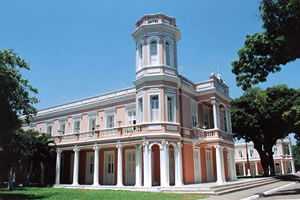
\includegraphics[width=16cm]{figuras/exemplo-1}
%		}{
%			\Fonte{\citeonline[p.~5]{UFC2012}.}
%		}	
%	\end{figure}
	
 %   Texto1 texto texto texto texto texto texto texto texto texto texto texto texto texto texto texto texto texto texto texto texto texto texto texto texto texto texto texto texto texto texto texto texto texto texto texto texto texto texto texto texto texto texto texto texto1.

%    Texto2 texto texto texto texto texto texto texto texto texto texto texto texto texto texto texto texto texto texto. Texto texto texto texto texto texto texto texto texto texto texto texto texto texto texto texto texto texto texto2.

 %   Texto3 texto texto texto texto texto texto texto texto texto texto texto texto texto texto texto texto texto texto. Texto texto texto texto texto texto texto texto texto texto texto texto texto texto texto texto texto texto texto3.

  %  Texto4 texto texto texto texto texto texto texto texto texto texto texto texto texto texto texto texto texto texto. Texto texto texto texto texto texto texto texto texto texto texto texto texto texto texto texto texto texto texto4.

 %   A Figura \ref{fig:sondas} texto texto texto texto texto texto texto texto texto texto texto texto texto texto texto texto texto texto texto. Texto texto texto texto texto texto texto texto texto texto texto texto texto texto texto texto texto texto texto3.

%	\begin{figure}[h!]
%		\centering
%		\captionsetup{width=14cm}%Da mesma largura que a figura
%		\Caption{\label{fig:sondas} Gráfico da atmosfera superior}	
%		\UFCfig{}{
%			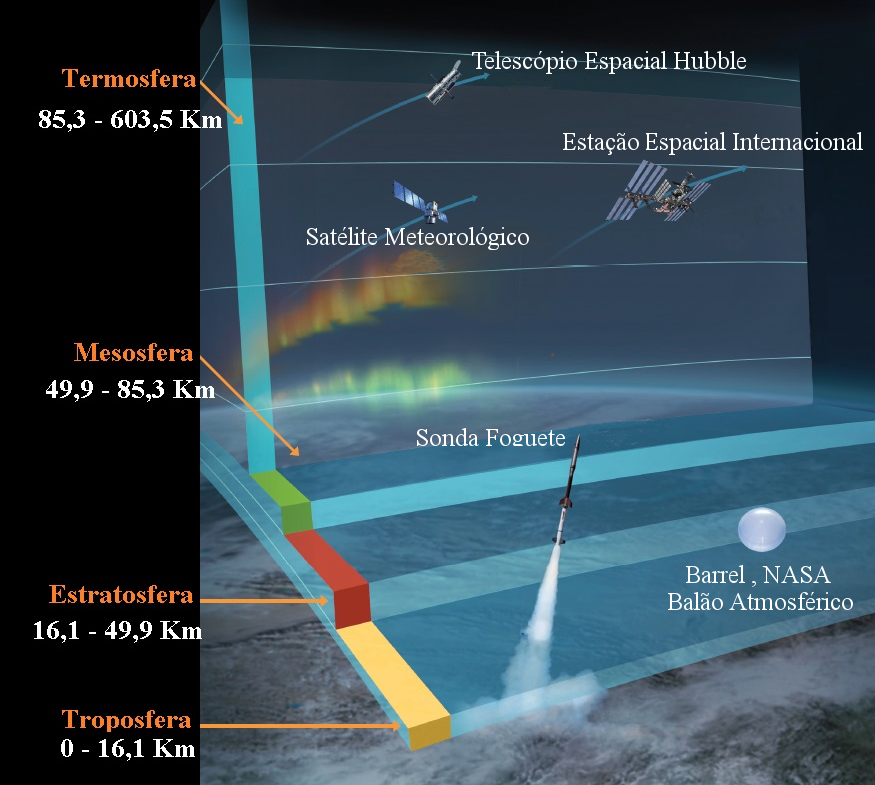
\includegraphics[width=14cm]{figuras/sondas}
%		}{
%			\Fonte{adaptado da \citeonline[p.~98]{NASA2016}.}}	
%	\end{figure}
%
 %   Texto5 texto texto texto texto texto texto texto texto texto texto texto texto texto texto texto texto texto texto texto texto texto texto texto texto texto texto texto texto texto texto texto texto texto texto texto texto texto texto texto texto texto texto texto texto5.

 %   Texto6 texto texto texto texto texto texto texto texto texto texto texto texto texto texto texto texto texto texto texto texto texto texto texto texto texto texto texto texto texto texto texto texto texto texto texto texto texto texto texto texto texto texto texto texto5.

 %   Texto7 texto texto texto texto texto texto texto texto texto texto texto texto texto texto texto texto texto texto texto texto texto texto texto texto texto texto texto texto texto texto texto texto texto texto texto texto texto texto texto texto texto texto texto texto texto texto texto texto texto texto texto texto texto texto texto texto texto texto texto texto texto texto texto6.

 %   Evite terminar seções, capítulos e etc com figura. Procure escrever mais.

%\section{Inserindo tabelas}\label{sec:tabelas}
    
%    A Tabela \ref{tab:exemplo-1}... texto texto texto texto texto texto texto texto texto texto texto texto texto texto texto texto texto texto texto. Texto texto texto texto texto texto texto texto texto texto texto texto texto texto texto texto texto texto texto.
	


	%\begin{table}[h!]	
	%	\centering
	%	\Caption{\label{tab:exemplo-1} Exemplo de tabela}	
	%	\UFCtab{}{
	%		\begin{tabular}{cll}
	%			\toprule
	%			Ranking & Exon Coverage & Splice Site Support \\
	%			\midrule \midrule
	%			E1 & Complete coverage by a single transcript & Both splice sites\\
	%			E2 & Complete coverage by more than a single transcript & Both splice sites\\
	%			E3 & Partial coverage & Both splice sites\\
	%			E4 & Partial coverage & One splice site\\
	%			E5 & Complete or partial coverage & No splice sites\\
	%			E6 & No coverage & No splice sites\\
	%			\bottomrule
	%		\end{tabular}
	%	}{
	%	\Fonte{elaborado pelo autor.}
	%}
	%\end{table}




  
%\subsection{Uso de siglas} \label{sec:siglas}

%    Para utilizar siglas, primeiro defina a sigla no arquivo "lista-de-abreviaturas-e-siglas"~ dentro da pasta "1-pre-textuais" com o comando 
%    \begin{verbatim}
 %       \newacronym{ABNT}{ABNT}{Associação Brasileira de Normas Técnicas}
 %   \end{verbatim}
%    Depois chame a sigla com o comando:
 %   \begin{verbatim}
%        \gls{ABNT}
%    \end{verbatim}
 %   Fica assim: \gls{ABNT}. A primeira vez que o comando é usado para uma determinada sigla, aparece o significado por extenso da sigla com a sua abreviação em seguida. A partir da segunda vez que o comando para uma determinada sigla é usado, aparace apenas a sigla. Por exemplo: \gls{ABNT}.  
    
 %   Veja o código fonte de outros exemplos: Teste de siglas \gls{TEST}, outros exemplos de siglas: \gls{DA}, \gls{MCEG}. 
  %  Repare que sempre as siglas estão sendo definidas primeiramente no arquivo ``lista-de-abreviaturas-e-siglas''.
    
%\subsubsection{Exemplo de subseção quaternária} \label{sec:quater}

%Texto texto texto texto texto texto texto texto texto texto texto texto texto texto texto texto texto texto texto texto texto texto texto texto texto texto texto texto texto texto texto texto texto texto texto texto texto texto texto texto texto texto texto texto texto.

%\subsubsubsection{Exemplo de subseção quinária} 

%Texto texto texto texto texto texto texto texto texto texto texto texto texto texto texto texto texto texto texto texto texto texto texto texto texto texto texto texto texto texto texto texto texto texto texto texto texto texto texto texto texto texto texto texto texto.

\nocite{ibge,introducao-ta, pcd-mercado-trabalho, abnt, laramara, secretaria, dorina, cadevi}

	\chapter{Gerenciamento do projeto}
\label{chap:metodologia}

    Ao iniciar o desenvolvimento de um novo projeto, é primordial definir um plano com etapas estabelecidas a fim de alcançar os objetivos gerais. Nesse sentido, a organização de prazos, o levantamento de compreensão dos papéis ocupados por cada integrante dentro da equipe, a designação de tarefas e a gestão de entregas constituem aspectos fundamentais para garantir um projeto final robusto e completo. Portanto, definir ferramentas e metodologias para guiar o gerenciamento desses aspectos mostra-se relevante para manter um progresso contínuo e sem conflitos.


\section{Metodologias e Ferramentas de Gestão de Projeto}\label{sec:exemplo-de-algoritmos-e-figuras}

    Com o propósito de manter entregas constantes e estabelecer um acesso fácil a todos os aspectos do projeto, decidiu-se utilizar as ferramentas fornecidas pela Atlassian devido às funcionalidades ofertadas e, sobretudo, pela centralização das informações e integração entre as diferentes plataformas. As plataformas são gratuitas para equipes com até dez membros, promovendo um alto custo-benefício ao grupo. 

    \subsection{Jira}
    
    O Jira foi estabelecido como a principal maneira de organizar e designar tarefas entre os integrantes do grupo. Por promover a possibilidade de visualizar itens pendentes em linhas do tempo, segmentar entregas semanais em tarefas atômicas e fornecer uma visão unificada de tudo que está pendente, em progresso ou concluído, a plataforma facilita a gestão eficiente do fluxo de trabalho.
    
    Além disso, a ferramenta permite que a equipe crie campos personalizados para atender às necessidades do projeto, acesse diferentes dashboards e utilize filtros para visualizações de diferentes aspectos do projeto. Com relatórios e métricas detalhadas, o Jira também oferece dados sobre o progresso do projeto, ajudando a identificar áreas de melhoria e de sucesso, auxiliando a tomar decisões informadas para impulsionar o sucesso do projeto.

    Por fim, o Jira oferece recursos adicionais, como a atribuição de prazos, a adição de descrições detalhadas às tarefas e a possibilidade de anexar arquivos relevantes, como documentos ou imagens. Isso contribui para uma comunicação mais eficiente entre os membros da equipe e auxilia na documentação do processo de desenvolvimento.

    \subsection{Adaptação do framework Scrum}

    O framework Scrum, conhecido por sua agilidade e flexibilidade, foi adaptado para se adequar ao contexto específico do projeto, levando em consideração a disponibilidade dos integrantes do grupo. Ao invés de adotar sprints com períodos de tempo fixos, decidiu-se estabelecer o ritmo de trabalho com base nos dias em que ocorrem as entregas em sala de aula. Essa abordagem permite uma melhor sincronização das atividades com o calendário acadêmico, garantindo que todas as tarefas estejam concluídas a tempo para as avaliações.

    Embora as aulas aconteçam semanalmente, as entregas podem ser espaçadas por períodos maiores, a depender do calendário acadêmico. Assim, optamos por agrupar todas as atividades necessárias para alcançar o objetivo da próxima entrega, independentemente do intervalo de tempo entre elas. Essa estratégia permite uma alocação mais eficiente de tempo e recursos, pois é possível focar nas tarefas mais relevantes e críticas para o avanço do projeto. Além disso, ao definir as sprints baseadas em entregas, viabiliza-se conversas com o professor durante as aulas anteriores à apresentação com o propósito de tirar dúvidas, refinar detalhes e coletar feedbacks sobre o andamento do projeto.
    
    No Jira, utilizamos a divisão por épicos para organizar e priorizar as diversas etapas e funcionalidades do projeto. Essa categorização nos permite visualizar de forma clara e detalhada todas as atividades que precisam ser realizadas até a data limite estabelecida. Com isso, podemos planejar e executar as tarefas de forma estratégica, mantendo o foco no cumprimento dos objetivos e na entrega bem-sucedida do projeto. Ademais, cada tarefa, sub-tarefa e história pode ser designada aos integrantes.

    \begin{figure}[h!]
        \captionsetup{width=1\textwidth} 
        \caption{\label{fig:epicos_jira} Divisão por épicos para organização de entregas}
        \centering
        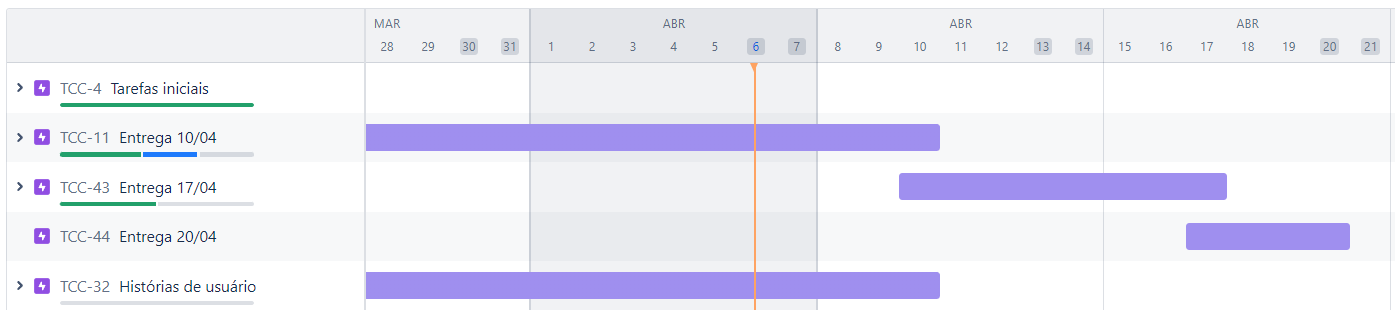
\includegraphics[width=1\textwidth]{figuras/epicos_jira}
        \caption*{Fonte: elaborada pelo autor.}
    \end{figure}

    A Figura \ref{fig:epicos_jira} ilustra a divisão por épicos, sendo que cada um constitui uma data de entrega. Assim, o intervalo de tempo das entregas ficam facilmente visíveis. 

    
    \subsection{Kanban}
    No contexto do projeto, a ferramenta de administração de produção Kanban foi adotada para facilitar o gerenciamento visual das tarefas, prioridades e fluxo de trabalho da equipe. O Kanban é uma metodologia ágil que se baseia em quadros visuais divididos em colunas que representam diferentes estágios do processo de trabalho. Cada tarefa é representada por um cartão, que é movido pelas colunas conforme progride no fluxo de trabalho.

    No presente projeto, a ferramenta Kanban foi implementada utilizando o Jira, uma plataforma que oferece recursos específicos para a criação e personalização de quadros Kanban. Esses quadros podem ser adaptados de acordo com as necessidades da equipe, permitindo a definição de colunas correspondentes aos estágios específicos do processo de desenvolvimento de software, como "A fazer", "Em andamento"  e "Concluído". A atualização das tarefas nos quadros é refletida instantaneamente quando o estado do trabalho é atualizado, evitando duplicação de itens em diferentes lugares, como ilustra a Figura \ref{fig:kanban}.
    
    A exibição dos itens nos quadros pode ser filtrada por épicos, mostrando a situação das tarefas de cada entrega, e também pode ser agrupada por épico, subtarefa ou responsável. Essas funcionalidades disponibilizadas pela plataforma facilitam o acompanhamento do progresso do projeto e permitem uma visão clara e organizada das atividades em andamento.

    \begin{figure}[h!]
        \captionsetup{width=1\textwidth}
        \caption{\label{fig:kanban} Quadros do Kanban disponibilizados no Jira}
        \centering
        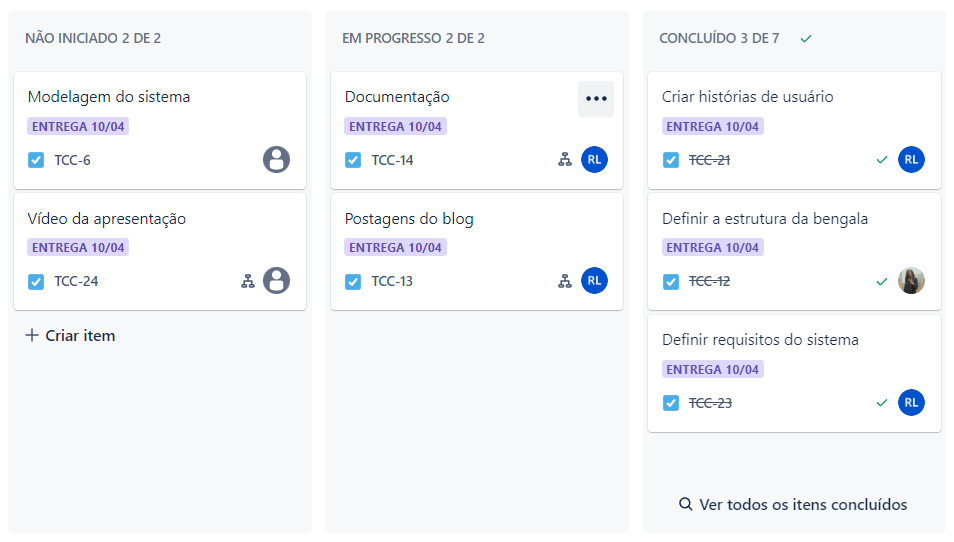
\includegraphics[width=1\textwidth]{figuras/kanban} 
        \caption*{Fonte: elaborada pelo autor.}
    \end{figure}

    \subsection{Github e Git}

    O GitHub, uma plataforma de hospedagem de arquivos baseada no sistema de versionamento Git, é uma ferramenta amplamente reconhecida e adotada pela comunidade de desenvolvimento de software. Sua popularidade se deve à sua capacidade de gerenciar alterações e facilitar a colaboração entre equipes de desenvolvimento. Para o projeto, a escolha do GitHub foi natural, uma vez que todos os membros já possuíam familiaridade com a plataforma.
    
    O Git, por sua vez, é um sistema de versionamento distribuído que permite que os membros de um projeto clonem o repositório, realizem alterações localmente e abram solicitações para mesclar essas mudanças na versão principal existente no repositório. Uma das principais vantagens do Git é sua capacidade de lidar com conflitos de maneira eficiente, permitindo que os desenvolvedores resolvam discrepâncias entre diferentes versões do código sem comprometer a estabilidade do projeto.
    
    Além disso, o Jira oferece integração com o GitHub. Isso significa que cada tarefa pode ser associada a uma nova \textit{branch} ou \textit{commit} no repositório, permitindo uma correlação direta entre o gerenciamento do projeto e o trabalho realizado pelo grupo de desenvolvimento.

    \subsection{Confluence}
    Por fim, o Confluence foi utilizado como uma ferramenta para centralizar o acesso à informação, de forma que documentos importantes possam ser facilmente visualizados na página inicial do Jira. Ele serve como um repositório onde documentos importantes, como requisitos do projeto, especificações técnicas de componentes e links de referência, são armazenados e facilmente acessíveis a todos os membros da equipe.
    
    Além disso, o Confluence possibilita a criação de páginas personalizadas e estruturadas de acordo com as necessidades do projeto. Isso permite que a equipe colabore na elaboração de documentos, adicione comentários, faça edições e revisões em tempo real. O acesso compartilhado auxilia na inclusão dos membros da equipe dentro das principais decisões do projeto.

    \section{Gestão da Comunicação}
    A gestão da comunicação é uma peça fundamental para o sucesso de qualquer projeto, pois envolve tanto a disseminação de informações dentro da equipe quanto a interação com as partes externas interessadas no projeto, como professores e colegas. Nesse contexto, foram utilizadas três ferramentas para viabilizar a interação entre esses dois públicos: o aplicativo de mensagens instantâneas WhatsApp para o diálogo entre a equipe, o blog para a publicação de atualizações acerca do projeto e um canal no YouTube para registro de apresentações e progresso do repositório.

    O blog, por ser uma plataforma pública facilmente acessível, é ideal para compartilhar informações e atualizações sobre o projeto com um público mais amplo. Nele, são compartilhadas atualizações sobre o andamento do projeto, planos de execução, desafios enfrentados pela equipe, mudanças de planos e objetivos alcançados. Além disso, o blog proporciona uma oportunidade promover a transparência no desenvolvimento do projeto, tanto para o professor avaliador quanto para alunos que estejam buscando por referências. As postagens são atualizadas semanalmente, com um resumo do que foi feito ao longo da semana por todos os integrantes, decisões tomadas, dificuldades observadas e o planejamento futuro do trabalho.
    
    Por outro lado, foi criado um grupo no WhatsApp como canal de comunicação interna assíncrona, utilizado para facilitar a troca rápida de mensagens entre os membros da equipe. Por ser uma plataforma de mensagens instantâneas, amplamente utilizada por todos os integrantes, o aplicativo permite uma comunicação ágil e direta, sendo útil para coordenar tarefas pendentes no Jira, discutir ideias, resolver problemas urgentes, manter todos os membros atualizados, informar sobre decisões e definir os próximos passos. Além disso, por ser acessível através de aplicativo mobile, via web e aplicação desktop,  a comunicação torna-se mais conveniente aos membros.
    
    A comunicação síncrona é realizada ao longo da semana, durante os encontros na faculdade, para resolver questões maiores e sensíveis acerca do projeto. Devido ao fato das rotinas dos integrantes serem divergentes por incompatibilidade de horário, reuniões tornam-se menos frequentes e são realizadas durante os finais de semana. Assim, a comunicação pelo grupo no WhatsApp e a atualização das tarefas no Jira tornam-se imprescindíveis.



    \section{Organização das tarefas}
    Em vez de atribuir responsabilidades específicas a cada integrante, foi optada a adoção de uma abordagem mais flexível, na qual todos os membros da equipe têm a oportunidade de contribuir em diferentes aspectos do projeto. A decisão foi fomentada pela prática de manter o código coletivo da metodologia ágil Extreme Programming (XP), que incentiva toda a equipe a conhecer todas as partes do sistema em vez de centralizar atribuições em integrantes específicos.

    Essa decisão foi tomada visando promover uma maior colaboração e um ambiente de trabalho mais inclusivo, no qual todos possam aprender e se desenvolver em diversas áreas. Além disso, essa abordagem permite que a equipe se adapte mais facilmente às mudanças de escopo e prioridades. Por fim, a escolha também foi adotada como uma estratégia para mitigar o risco de dependência excessiva de um único membro da equipe em uma área específica, reduzindo assim o impacto potencial caso um integrante decida deixar o projeto. 
    
    Ao permitir que todos os integrantes tenham experiência em várias áreas, também estamos capacitando-os a serem mais versáteis e preparados para lidar com desafios diversos que possam surgir ao longo do desenvolvimento do projeto.
    
    Apesar disso, garantir que existam pessoas acompanhando cada etapa do projeto é fundamental para uma gestão de todos os aspectos do projeto, garantindo sua conclusão dentro do prazo estabelecido, mantendo a qualidade do trabalho realizado e fornecendo um suporte aos integrantes. Essa atribuição de responsabilidades não implica em limitar o conhecimento ou participação dos demais membros da equipe, mas sim em criar uma estrutura de suporte e organização que facilite a gestão eficiente das tarefas e a tomada de decisões ao longo do projeto.


    \section{Segmentação do Projeto}
    O projeto foi segmentado em duas vertentes principais: o desenvolvimento da bengala e a gestão do projeto. Cada uma dessas áreas foi subdividida em categorias específicas, designando um ou mais integrantes para supervisionar o cumprimento de prazos, estabelecer as tarefas necessárias para cada entrega e monitorar o progresso geral.

    \subsection{Desenvolvimento da Bengala}
    Esta vertente concentra-se na concepção, design e implementação da bengala inteligente. Envolve a seleção e integração dos componentes eletrônicos, testes e validações do sistema, desenvolvimento do software embarcado,  entre outras atividades relacionadas diretamente à criação da bengala inteligente.


    \begin{itemize}
        \item \textbf{Modelagem física:} Refere-se à criação de modelos físicos, protótipos e desenhos técnicos da bengala inteligente. Abrange as decisões de design do produto, questões de ergonomia, usabilidade e integração dos componentes eletrônicos no produto final.
        
        \item \textbf{Seleção e teste dos componentes:} Envolve a escolha dos componentes eletrônicos que serão utilizados na bengala inteligente, levando em consideração requisitos de desempenho, custo, disponibilidade e compatibilidade. Além disso, compreende teste e validação dos componentes para garantir que atendam aos requisitos do projeto.
        
        \item \textbf{Desenvolvimento do software embarcado:} Refere-se ao desenvolvimento do código que irá operar a bengala, incluindo a configuração dos componentes, processamento dos dados concebidos pelos sensores e implementação de funcionalidades específicas.
        
        \item \textbf{Montagem do circuito:} Esta etapa envolve a montagem física dos componentes eletrônicos na bengala inteligente, incluindo a soldagem de componentes em placas de circuito, conexão de fios e cabos, e montagem de outros elementos necessários para o funcionamento do sistema eletrônico.
        
        \item \textbf{Documentação:} Consiste na elaboração de registros detalhados de todas as etapas do projeto, desde a definição inicial das especificações da bengala até a documentação final do produto. Isso inclui a definição do escopo do projeto, a documentação das decisões de design, a descrição dos requisitos funcionais e não funcionais, apresentação da arquitetura do sistema e criação de manuais de usuário.
    \end{itemize}

    \subsection{Gestão do Projeto}
    A vertente de gestão do projeto engloba uma série de tarefas secundárias essenciais para o bom andamento e organização das atividades relacionadas ao desenvolvimento da bengala inteligente. Nesta área, as atividades são paralelas ao desenvolvimento e incluem postagens no blog, edição de vídeos, gerenciamento do canal no YouTube, formatação dos documentos em LaTeX, apresentação de slides e gestão geral do projeto.


    \begin{itemize}
        \item \textbf{Blog:} Compreende as funções de criar, manutenir e postar frequentemente as atualizações no blog, incluindo todas as atividades realizadas pela equipe. Envolve a comunicação com a equipe para entender o que foi feito e sintetizar o progresso, mudanças de planos e reuniões nas postagens para comunicar à audiência externa acerca do avanço do projeto.
        
        \item \textbf{Edição dos vídeos e gestão do canal no YouTube:} Envolve a produção, edição e postagem dos vídeos produzidos ao longo do projeto no canal do YouTube. Engloba os vídeos de apresentação do projeto, demonstração da bengala e evolução de commits no repositório do GitHub.
        
        \item \textbf{LaTeX:} Integra a padronização e formatação adequada dos documentos produzidos a respeito da bengala inteligente, incluindo desenho da aplicação, documentos de pesquisa e especificação do sistema. Esse segmento inclui o uso de normas voltadas à produção de textos acadêmicos estabelecidas pela Associação Brasileira de Normas Técnicas (ABNT).
        
        \item \textbf{Apresentação de slides:} Trata-se da área relacionada à criação dos slides necessários para as apresentações de cada etapa do projeto, seguindo o modelo proposto pela instituição de ensino. Inclui a leitura, compreensão e sintetização dos documentos produzidos como base para o desenvolvimento do projeto.
        
        \item \textbf{Gestão geral do projeto:} Relaciona-se ao acompanhamento das tarefas do projeto, supervisão das métricas no Jira, divisão equilibrada de trabalho entre os integrantes e acompanhamento dos gastos do projeto. O propósito é gerenciar o andamento das atividades como um todo, garantindo que tudo tenha sido feito a cada entrega.
    \end{itemize}

    \section{Papéis}
    
    Considerando as duas vertentes principais do trabalho e suas sub-tarefas, foi atribuída a uma ou mais pessoas a responsabilidade de gerenciar as atividades relacionadas a cada área específica. Para determinar quantas pessoas seriam necessárias por setor, o grupo estabeleceu critérios com base no grau de dificuldade e importância para o projeto, a fim de mitigar riscos futuros.
    
    Dessa forma, embora todos os integrantes possam participar de várias atividades, foi definido quais ocupariam os papéis de gerenciamento em cada área do projeto. Essa distribuição de responsabilidades visa garantir uma gestão eficaz e focada em cada aspecto essencial do trabalho.

    \subsection{Desenvolvimento da Bengala}

    Para a efetiva implementação das tarefas necessárias à execução do projeto, os papéis foram distribuídos a partir da participação integral dos integrantes na decisão. Assim, os critérios para a atribuição dos papéis incluem aptidão dos membros e nível de complexidade das tarefas, já que atividades mais sensíveis exigiam mais pessoas para a garantia de execução.
    
    O Quadro 2 ilustra a distribuição das tarefas de desenvolvimento da bengala entre os cinco integrantes do grupo, divididas em cinco principais divisões voltadas à implementação do projeto: modelagem física, seleção e teste dos componentes, desenvolvimento do software, montagem do circuito e documentação.
    
        \begin{quadro}[!ht]    
            \captionsetup{width=1.0\textwidth} % Definindo a largura da legenda
            \caption{Atribuição dos papéis para atividades de desenvolvimento da bengala}    
            \begin{tabular}{lrrrrrr}
                \toprule
                Atividades & Ana Paula & Eduardo & Felipe  & Paulo & Raissa \\
                \midrule
                Modelagem física                        &   & X & X  &   &   \\
                Seleção e teste dos componentes         &   &   &   &   & X \\
                Desenvolvimento do software             &   &   &  & X & X \\
                Montagem do circuito                    &   & X &    & X &   \\
                Documentação                            & X &   &    &   & X \\
                \bottomrule
            \end{tabular}
            \caption*{Fonte: elaborada pelos autores.} % Legenda sem rótulo
        \end{quadro}

    A tabela acima ilustra a divisão clara de responsabilidades para as etapas essenciais do projeto de desenvolvimento da bengala, garantindo uma abordagem coordenada e eficiente ao longo de todas as fases de implementação.
   
    \subsection{Gestão do Projeto}
    Para garantir uma execução eficiente e organizada do projeto, foram atribuídos papéis específicos aos membros da equipe com base em suas habilidades e na natureza das atividades. 
        \begin{quadro}[!ht]    
            \captionsetup{width=1.0\textwidth} % Definindo a largura da legenda
            \caption{Atribuição dos papéis para atividades de gestão do projeto}    
            \begin{tabular}{lrrrrrr}
                \toprule
                Atividades & Ana Paula & Eduardo & Felipe & Paulo & Raissa \\
                \midrule
                Blog                                &   &   &     &   & X \\
                Edição de vídeos e YouTube          &   & X &   &      &   \\
                LaTeX                               & X &   &   &      &   \\
                Slides                              &   &   & X &      &   \\
                Gestão gera                         &   &   &   &      & X \\
                \bottomrule
            \end{tabular}
            \caption*{Fonte: elaborada pelos autores.} % Legenda sem rótulo
        \end{quadro}
        O Quadro 2 apresenta a distribuição das responsabilidades de gestão entre os integrantes do grupo, abrangendo desde a administração do blog e edição de vídeos até a elaboração de documentos em LaTeX e preparação de apresentações. Essa estratégia não apenas facilita a coordenação das tarefas, mas também assegura uma abordagem colaborativa e integrada ao longo do desenvolvimento do projeto.




	\chapter{Desenvolvimento do Projeto}
\label{chap:resultados}

    A etapa de desenvolvimento do projeto desempenha um papel abrangente, contudo, extremamente crucial para a transformação de ideias em aplicações práticas, como definição do escopo do projeto, histórias de usuários, requisitos funcionais e não funcionais, definição de tecnologias e estabelecimento da arquitetura do modelo. Um estabelecimento robusto desses aspectos, ainda na etapa inicial do desenvolvimento, evita conflitos de requisitos no futuro ou impossibilidade de implementação do projeto devido à falta de clareza no escopo do projeto.   

\section{Escopo do Projeto}
\label{sec:resultados-do-experimento-a}

    A bengala inteligente é uma ferramenta de TA que busca auxiliar usuários com deficiência visual a se locomover com mais independência e autonomia pelo espaço. O acoplamento de um microcontrolador e diferentes sensores na bengala fornecem ao usuário uma maior noção do ambiente, a fim de devolver capacidades funcionais prejudicadas no campo da visão.

    \subsection{O que a bengala inteligente é?}
    A seguir, serão apresentados os principais aspectos da bengala inteligente, incluindo sua definição como ferramenta de assistência para pessoas com deficiência visual e os requisitos funcionais em sistemas embarcados.
        \begin{itemize} 
            \item Uma ferramenta de assistência para pessoas com deficiência visual, projetada para melhorar a mobilidade e a independência.
            
            \item Capaz de detectar obstáculos sólidos e outros elementos do ambiente que possam representar riscos à segurança.
            
            \item Equipada com sensores que fornecem feedback tátil ou auditivo ao usuário, permitindo uma navegação mais eficiente e segura.
            
            \item Projetada para ser leve, fácil de usar e confortável durante o uso prolongado.
            
            \item Voltada para garantir uma longa duração da bateria.
        \end{itemize}

\section{Design da bengala}
O design da bengala foi cuidadosamente desenvolvido para minimizar a interferência dos componentes eletrônicos nas funções e no uso original da bengala tradicional. As dimensões da caixa eletrônica foram projetadas para alterar o mínimo possível as medidas originais, facilitando a adaptação do usuário ao novo modelo. A caixa possui um furo central, permitindo que o elástico da bengala continue passando de uma extremidade à outra, preservando a característica dobrável da bengala e mantendo sua funcionalidade prática, onde ela se monta automaticamente ao ser desdobrada.

Essas adaptações permitem que todos os componentes eletrônicos fiquem concentrados no segmento do cabo. Isso possibilita que, futuramente, apenas o cabo seja vendido, permitindo a adaptação a uma bengala já em uso, que o usuário possa preferir por outras adaptações, como uma ponta de rolamento ou cores indicativas. Essa decisão também mantém o peso adicional próximo à mão do usuário, facilitando o movimento da ponta da bengala de um lado para o outro, devido ao efeito de alavanca.

O formato do cabo será alterado de circular para elíptico. Essa mudança tem como objetivo facilitar o alinhamento dos sensores, que devem estar sempre apontados para frente e para cima. Com um cabo elíptico e um relevo indicador, o usuário pode segurar a bengala com a palma da mão voltada para cima ou para baixo, garantindo o alinhamento correto dos sensores, mesmo com perda total de visão, sem exigir um esforço adicional para encontrar o alinhamento adequado. Essa solução foi inspirada no design de cabos de espadas, que são elípticos ou retangulares para auxiliar no alinhamento.

O sensor, ao detectar proximidade com uma superfície ou objeto à altura da mão, acionará um motor vibrador embutido no cabo, alertando o usuário sobre a presença de um obstáculo que possa ter sido ignorado pela ponta da bengala. As vibrações aumentam em frequência à medida que a distância do obstáculo diminui.

O cabo contará com uma superfície sensível ao toque, que, em conjunto com um sensor interno, detecta o contato da mão. Quando o sistema estiver ligado, essa conexão previne a perda da bengala; caso ocorra a separação do usuário, após alguns segundos, um alarme sonoro será acionado para ajudar o usuário a encontrar a bengala, mesmo em condições de pouca ou nenhuma visibilidade. O sistema também será de fácil ativação e desativação por meio de um botão de acesso rápido no cabo.

As decisões de preservar o design original e minimizar as alterações foram baseadas nas experiências de pessoas com deficiência visual e na observação de como a bengala é utilizada no cotidiano, garantindo uma transição suave e eficiente para o novo modelo assistivo.

\section{Requisitos Funcionais}
    Requisitos funcionais em sistemas embarcados definem as funcionalidades específicas que o sistema deve realizar, levando em conta as limitações de recursos do hardware. Dessa forma, estabelece as funcionalidades que a bengala fornece ao usuário e como o processamento de dados captados por sensores devem ser tratados.


\begin{quadro}[!ht]    
    \captionsetup{width=1.0\textwidth} % Definindo a largura da legenda
    \caption{Requisitos funcionais da bengala inteligente}  
    \renewcommand{\arraystretch}{1.5} % Aumenta o espaçamento entre as linhas
    \begin{tabular}{p{0.1\textwidth}p{0.2\textwidth}p{0.6\textwidth}} % Definindo larguras para as colunas
        \toprule
        Referência & Nome & Descrição \\
        RF01 & Identificação de objetos & A bengala deve ser capaz de detectar objetos sólidos, como paredes, móveis ou obstáculos, a uma distância de pelo menos um metro em relação aos sensores.   \\
        RF02 & Altura de objetos  & A bengala deve conseguir identificar objetos em diferentes alturas. \\
        RF03 & Detecção em ambientes escuros  &  A bengala deve ser capaz de identificar objetos independentemente da iluminação do local.  \\
        RF04 & Modo de vibração  &  A intensidade da vibração deve variar de acordo com a distância do objeto identificado, de forma que a vibração aumente conforme a distância diminui.  \\
        RF05 & Diferença entre os modos de vibração  & A alternância de intensidade deve ser perceptível ao usuário. \\
        RF06 & Recarregamento da bengala  & A bengala deve ser recarregável.  \\
        RF08 & Desligamento  & A bengala deve possuir um interruptor/botão para que seja desligada. \\
        \bottomrule
    \end{tabular}
    \caption*{Fonte: elaborada pelos autores.} % Legenda sem rótulo
\end{quadro}

    Os detalhes apresentados no Quadro 4 descrevem as funcionalidades de cada um dos requisitos funcionais da bengala, desde os aspectos básicos de detecção de objetos até as instruções de como deve funcionar o desligamento.

    
\section{Requisitos Não Funcionais}
    Os requisitos não funcionais se concentram em qualidades do sistema além das funcionalidades diretas. Isso pode incluir restrições de desempenho, consumo de energia pela bengala, latência de resposta, especificações técnicas, compatibilidade entre componentes e tamanho do conjunto de hardware.


\begin{quadro}[!ht]    
    \captionsetup{width=1.0\textwidth} % Definindo a largura da legenda
    \caption{Requisitos não funcionais da bengala inteligente}  
    \renewcommand{\arraystretch}{1.5} % Aumenta o espaçamento entre as linhas
    \begin{tabular}{p{0.1\textwidth}p{0.2\textwidth}p{0.6\textwidth}} % Definindo larguras para as colunas
        \toprule
        Referência & Nome & Descrição \\
        RNF01 & Tempo de vibração & O tempo entre a detecção de um objeto e o alarme através do motor de vibração não pode ser superior a um segundo.   \\
        RNF02 & Tempo de detecção  & A detecção dos objetos deve ocorrer em tempo real. \\
        RNF03 & Precisão  &  A identificação de objetos deve ser precisa e confiável, sem falsos positivos ou negativos.  \\
        RNF04 & Integração ergonômica  &  Os componentes e módulos devem ser integrados na bengala de forma discreta.  \\
        RNF05 & Entrada do carregador  & A entrada para recarregar a bengala deve ser compatível com os cabos facilmente encontrados no mercado, como USB-C ou Micro USB. \\
        RNF06 & Proteção contra sobrecarga  & A recarga não deve oferecer riscos à bateria ou ao usuário, devendo existir uma proteção contra superaquecimento ou sobrecarga.  \\
        RNF07 & Autonomia de bateria  &  A bateria deve durar, no mínimo, 8 horas entre cada recarga. \\
        RNF08 & Resistência da entrada  & A entrada do carregador deve ser resistente e fixa na estrutura da bengala. \\
        RNF09 & Conforto  &  A bengala deve possuir apoio de mão e ponteira.  \\
        RNF10 & Distribuição do peso &  O peso da bengala deve ser distribuído ao longo da extensão ou estar concentrado próximo ao apoio de mão.  \\
        RNF11 & Informações na bengala &  Todas as informações, como o indicador de ligado/desligado, devem estar escritas em Braille.  \\
        \bottomrule
    \end{tabular}
    \caption*{Fonte: elaborada pelos autores.} % Legenda sem rótulo
\end{quadro}

No Quadro 5, os requisitos não funcionais da bengala são esclarecidos, abordando aspectos como conforto, resistência, precisão de medição e ergonomia.

\section{Histórias de usuário}

    Histórias de usuário são projetadas para capturar requisitos de forma simples e compreensível. Cada história de usuário descreve uma funcionalidade do sistema do ponto de vista do usuário final, fornecendo contexto sobre o que precisa ser feito e por que é importante. Essas histórias são essenciais para manter o foco nas necessidades dos usuários durante todo o ciclo de desenvolvimento, ajudando a equipe a priorizar e planejar suas atividades de forma eficaz. Ao descrever os requisitos em termos de histórias de usuário, as equipes podem garantir que estão construindo as funcionalidades certas para satisfazer as necessidades reais dos usuários finais.
    
    O processo de desenvolver as histórias permite que a equipe possa visualizar os requisitos em termos práticos. Ademais, a elaboração de critérios de aceitação para cada requisito auxilia o processo de teste e validação das funcionalidades, uma vez que define em termos práticos o que deve ser alcançado para que o desenvolvimento seja considerado bem-sucedido.

    A seguir, serão apresentadas as histórias de usuário da bengala, estabelecidas com base na revisão bibliográfica de trabalhos anteriores, bem como os seus respectivos critérios de aceitação.

    \subsection{Recarregamento da Bengala}
    \begin{quote}
    \textit{"Como usuário, preciso que recarregar a bengala seja um processo simples e conveniente, garantindo sua prontidão para uso sempre que necessário e evitando que fique inutilizada devido à falta de carga."}
    \end{quote}    
    \noindent\textbf{Critérios de Aceitação:}
    \begin{itemize}
        \item O processo de recarga deve ser simples e intuitivo, exigindo apenas uma conexão fácil entre a bengala e a fonte de energia, como um cabo USB ou um adaptador de energia.
        \item A bengala deve possuir uma entrada para um cabo simples de ser encontrado no mercado, como micro USB, USB-C ou USB.
        \item Deve haver um indicador sonoro que informe ao usuário quando a bateria estiver completamente carregada, para garantir que o processo de recarga seja concluído com sucesso.
        \item O tempo necessário para recarregar a bateria da bengala deve ser razoável e adequado para o uso diário, evitando longos períodos de espera para que o dispositivo esteja pronto para uso novamente.
        \item O conector da bengala deve ser resistente, a fim de que suporte múltiplas conexões e desconexões ao longo do tempo sem entortar, quebrar, afundar ou parar de funcionar.
        \item O processo de recarga deve ser seguro e protegido contra sobrecarga, curto-circuito ou superaquecimento, para evitar danos à bateria ou riscos para o usuário durante o carregamento.
        \item A bateria da bengala deve ter autonomia e durar, ao menos, 8 horas entre cada recarga.
    \end{itemize}

    \subsection{Resposta tátil}
    \begin{quote}
    \textit{"Como usuário, desejo que a vibração da bengala forneça uma resposta tátil que indique a distância dos objetos dos quais estou me aproximando."}
    \end{quote}    
    \noindent\textbf{Critérios de Aceitação:}
    \begin{itemize}
        \item Quando um objeto estiver a uma distância segura, a vibração da bengala deve ser suave e contínua.
        \item À medida que o usuário se aproxima de um objeto, a intensidade ou frequência da vibração deve aumentar gradualmente, indicando a proximidade.
        \item Quando o usuário estiver a uma distância perigosa ou muito próxima do objeto, a vibração deve ser forte e intermitente, alertando-o para uma possível colisão.
        \item A resposta tátil da bengala deve ser clara e compreensível, permitindo que o usuário interprete facilmente a distância dos objetos ao seu redor.
    \end{itemize}
        
    \subsection{Detecção de objetos}
    \begin{quote}
    \textit{"Como usuário, preciso que a bengala possa identificar objetos à frente para que eu permaneça seguro."}
    \end{quote}    
    \noindent\textbf{Critérios de Aceitação:}
    \begin{itemize}
        \item A bengala deve ser capaz de detectar objetos sólidos, como paredes, móveis ou obstáculos, a uma distância segura de pelo menos um metro à frente do usuário.
        \item A bengala deve conseguir identificar objetos em diferentes alturas.
        \item A identificação de objetos deve ser precisa e confiável, evitando falsos positivos ou negativos.
        \item Quando um objeto for detectado, a bengala deve fornecer um alerta imediato ao usuário, seja por meio de vibração, som ou outro meio de feedback sensorial.
        \item A detecção de objetos deve ocorrer em tempo real, permitindo que o usuário reaja rapidamente para evitar colisões ou acidentes.
        \item A bengala deve ser capaz de identificar objetos em diferentes condições de iluminação, garantindo sua eficácia tanto durante o dia quanto à noite.
        \item O sistema de identificação de objetos deve ser integrado de forma discreta e ergonômica à bengala, sem comprometer sua funcionalidade ou conforto para o usuário.
    \end{itemize}

    \subsection{Resistência à água}
    \begin{quote}
    \textit{"Como usuário, gostaria que a bengala fosse resistente à água para que eu possa sair com ela mesmo com chuva."}
    \end{quote}    
    \noindent\textbf{Critérios de Aceitação:}
    \begin{itemize}
        \item Os materiais utilizados para construir a bengala devem ser resistentes à água e que não absorvam umidade.
        \item Os componentes elétricos (incluindo microcontrolador, componentes e fios) devem estar armazenados em um recipiente vedado.
    \end{itemize}
        
    \subsection{Portabilidade}
    \begin{quote}
    \textit{"Como usuário, gostaria que a bengala fosse leve e fácil de usar, para que não seja exaustivo manter o uso por um longo período de tempo."}
    \end{quote}    
    \noindent\textbf{Critérios de Aceitação:}
    \begin{itemize}
        \item A bengala deve possuir dimensões similares às de outras bengalas encontradas no mercado.
        \item A bengala deve ser leve o suficiente para que não seja cansativo utilizá-la e mantê-la inclinada durante o uso.
    \end{itemize}
                
    \subsection{Desligar circuito}
    \begin{quote}
    \textit{"Como usuário, desejo poder desligar a bengala para que não permaneça desnecessariamente ligada enquanto não estiver sendo utilizada."}
    \end{quote}    
    \noindent\textbf{Critérios de Aceitação:}
    \begin{itemize}
        \item A bengala deve possuir um mecanismo de desligamento fácil, como um interruptor físico ou um botão de desligamento.
        \item O botão ou interruptor de desligamento deve ser mapeado na bengala de forma tátil, utilizando braille ou outra indicação tátil.
        \item Quando desligada, a bengala não deve consumir energia da bateria para garantir uma vida útil prolongada desta.
        \item O desligamento da bengala deve ser confirmado por meio de um indicador sonoro para garantir que o usuário saiba quando a bengala está realmente desligada.
        \item O processo de ligar e desligar a bengala deve ser rápido e conveniente, sem a necessidade de procedimentos complicados ou demorados.
        \item O mecanismo de desligamento deve ser robusto e confiável, com um design que evite desligamentos acidentais durante o uso normal da bengala.
        \item O desligamento da bengala não deve afetar negativamente outras funcionalidades ou operações desta, garantindo uma transição suave entre os estados ligado e desligado.
    \end{itemize}
                        
    \subsection{Conforto}
    \begin{quote}
    \textit{"Como usuário, preciso que a bengala seja confortável durante o uso, de forma que os componentes eletrônicos adicionais não a tornem mais desconfortável que uma bengala analógica comum."}
    \end{quote}    
    \noindent\textbf{Critérios de Aceitação:}
    \begin{itemize}
        \item O peso da bengala deve ser distribuído ao longo da extensão ou estar concentrado próximo à mão do usuário, para que não exija muito torque durante a utilização.
        \item A bengala deve possuir apoio de mão e ponteira.
        \item A adição dos componentes não pode ocupar um espaço excessivo no corpo da bengala.
    \end{itemize}

    \section{Componentes}
    É fundamental considerar uma variedade de fatores ao escolher os elementos que comporão o projeto. Além da disponibilidade das peças no mercado, é essencial avaliar o valor e o desempenho de cada componente dentro do propósito funcional da bengala. 

    \subsection{Módulo Motor de vibração}
    O motor de vibração está integrado a um módulo que conta com dois pinos de alimentação e um de entrada. Esse design permite que o módulo receba uma tensão variável, ajustando assim a intensidade da resposta vibratória do motor conforme necessário.

    Com capacidade para alcançar até 9000 rotações por minuto (RPM), o motor é responsável por gerar a sensação de vibração percebida pelo usuário. Essa característica torna o módulo ideal para controlar a resposta tátil do usuário com base na detecção de obstáculos próximos.
    
    
     \begin{figure}[h!]
        \captionsetup{width=1\textwidth}
        \caption{\label{fig:motorvibracao} Módulo do Motor de Vibração}
        \centering
        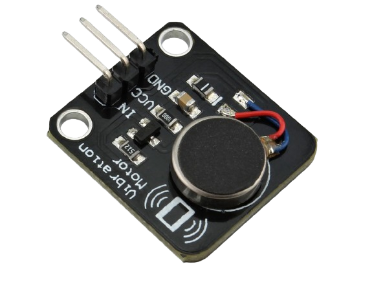
\includegraphics[width=0.3\textwidth]{figuras/motorvibracao} 
        \caption*{Fonte: Mercado Livre}
    \end{figure}

    O módulo recebe uma tensão de até 5V na porta digital para ativar o motor. Além disso, é possível controlar a frequência da vibração por meio do envio de pulsos rápidos para o módulo pela porta digital. A Figura \ref{fig:motorvibracao} ilustra o módulo, com três pinos e o motor de vibração.

    \subsection{Módulo Sensor de Distância Ultrassônico HC-SR04}

    O sensor ultrassônico, exibido na Figura \ref{fig:hcsr04}, desempenha uma função essencial ao detectar a distância entre o usuário e os objetos circundantes. Essa capacidade permite fornecer um feedback preciso sobre a localização e proximidade dos obstáculos. 

     \begin{figure}[ht]
        \captionsetup{width=1\textwidth}
        \caption{\label{fig:hcsr04} Módulo Sensor de Distância Ultrassônico HC-SR04}
        \centering
        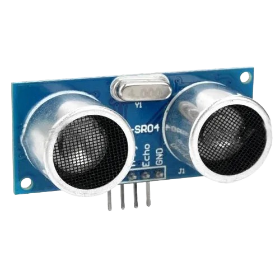
\includegraphics[width=0.3\textwidth]{figuras/hcsr04} 
        \caption*{Fonte: RoboCore}
    \end{figure}

    Este modelo de sensor destaca-se pela sua acessibilidade e possui um alcance efetivo de até quatro metros de distância em relação aos objetos detectados.   

    \subsection{Sensor Capacitivo Touch TTP223B}

    O sensor capacitivo \textit{touch}, localizado na área de aderência da Bengala Inteligente, oferece uma interação intuitiva para o usuário. Ao detectar o toque, a Bengala permanece no mesmo estado normal de funcionamento, detectando obstáculos e vibrando. No entanto, caso o sensor não detecte nenhum toque por um período determinado, ele ativará um alarme sonoro, permitindo que o usuário encontre a bengala ou a desligue caso tenha sido deixada ligada inadvertidamente. 



     \begin{figure}[h!]
        \captionsetup{width=1\textwidth}
        \caption{\label{fig:touch}Sensor Capacitivo \textit{Touch} TTP223B}
        \centering
        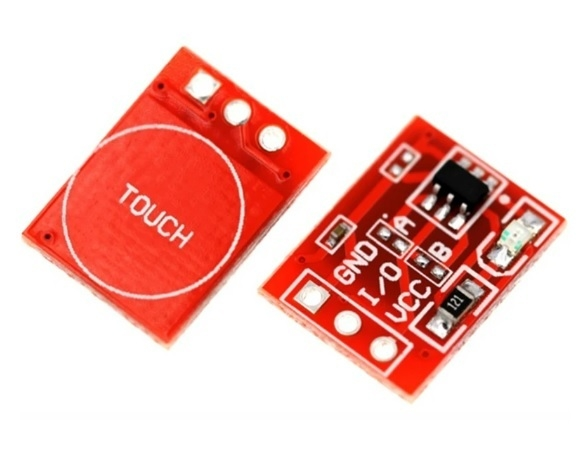
\includegraphics[width=0.3\textwidth]{figuras/touch} 
        \caption*{Fonte: Mercado Livre}
    \end{figure}

    Sensores de toque funcionam como uma chave, de forma que ativem um circuito elétrico e permitam o fluxo da corrente caso algum toque seja identificado. A Figura \ref{fig:touch} ilustra um sensor de toque no modelo TTP223B.
    
    
    \subsection{Chave DIP \texit{Switch}}
    O componente Chave DIP \texit{Switch} 1 Via, demonstrado na Figura \ref{fig:chave}, é responsável por controlar as funcionalidades da bengala inteligente, permitindo ao usuário ligar e desligar os recursos de acordo com suas necessidades. Com a simples alteração da posição da chave, é possível ativar ou desativar as funções da bengala de forma conveniente.

    É um componente que controla o circuito de forma fácil e de baixo custo, além de se adequar melhor ao projeto em relação a um botão por conta da possibilidade de identificar, pelo toque, se a chave está na posição ligada ou desligada.

    \begin{figure}[h!]
        \captionsetup{width=1\textwidth}
        \caption{\label{fig:chave}Chave DIP \texit{Switch} 1 Via}
        \centering
        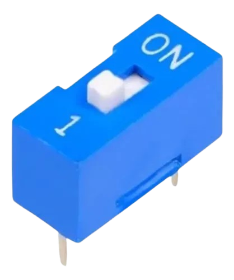
\includegraphics[width=0.3\textwidth]{figuras/chave} 
        \caption*{Fonte: Eletronik LV}
    \end{figure}

    \subsection{Módulo Buzzer Ativo}
    O \textit{buzzer} ativo desempenha um papel crucial na bengala inteligente ao ser o componente responsável pela emissão sonora, importante como meio de resposta ao usuário com algum grau de deficiência visual. Ele fornece alertas ao usuário quando o sensor de toque não recebe sinais após algum tempo, aprimorando a experiência de uso com a bengala. Seu som nítido e audível garante que informações importantes sejam transmitidas de forma clara e eficaz.


       \begin{figure}[h!]
        \captionsetup{width=1\textwidth}
        \caption{\label{fig:buzzer}Módulo Buzzer Ativo}
        \centering
        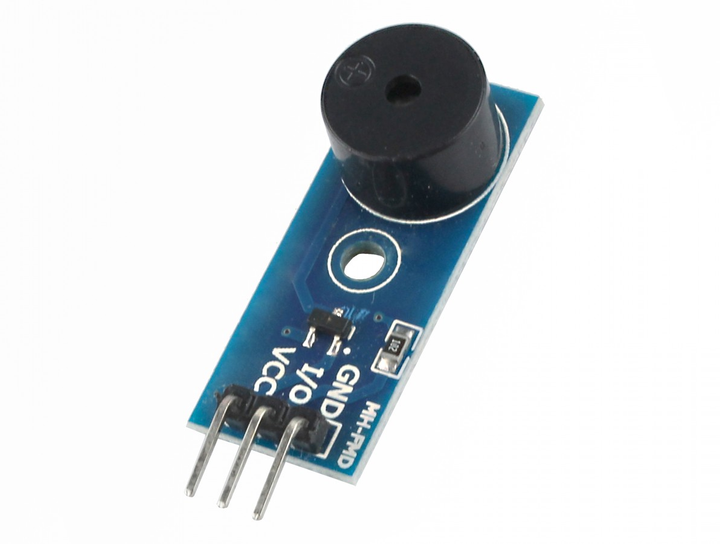
\includegraphics[width=0.4\textwidth]{figuras/buzzer} 
        \caption*{Fonte: A2 Robotics}
    \end{figure}

    A preferência ao \textit{buzzer} ativo justifica-se pela simplicidade de uso e pela ausência de necessidade de emitir diferentes frequências. Similar ao som emitido por micro-ondas, a resposta do \textit{buzzer} ativo acontece quando o módulo é energizado com uma tensão de até 5V. Dessa forma, não existe a necessidade de especificar o seu funcionamento de forma detalhada no código. 
    
    \subsection{Protoboard}
    A protoboard é um elemento fundamental na construção da bengala inteligente, oferecendo um ambiente flexível e seguro para a conexão dos componentes eletrônicos. Com sua matriz de furos e trilhas condutoras, a protoboard permite a prototipagem e teste dos circuitos de forma prática e versátil, sem necessidade de soldagem. É nesse espaço que os componentes são interligados e ajustados, proporcionando um ambiente propício para o desenvolvimento e aprimoramento da bengala inteligente.

    \begin{figure}[h!]
        \captionsetup{width=1\textwidth}
        \caption{\label{fig:protoboard} Protoboard de 400 furos}
        \centering
        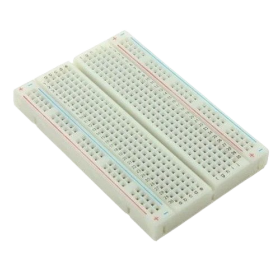
\includegraphics[width=0.3\textwidth]{figuras/protoboard} 
        \caption*{Fonte: Mercado Livre}
    \end{figure}

    \subsection{Microcontrolador}
    A placa Uno R3 é o componente-chave da bengala inteligente, responsável pelo controle e processamento das funcionalidades do dispositivo. É uma peça fundamental para que os sensores consigam ser gerenciados de maneira eficiente. 

    O modelo Uno é equipado com várias portas digitais e analógicas, além de possuir um tamanho compacto, facilitando a montagem de circuitos com integração de diferentes módulos.

    \begin{figure}[h!]
        \captionsetup{width=1\textwidth}
        \caption{\label{fig:arduino} Arduino Uno R3}
        \centering
        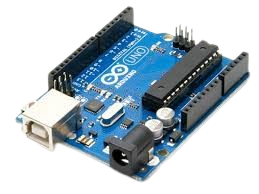
\includegraphics[width=0.3\textwidth]{figuras/arduino} 
        \caption*{Fonte: Fábrica de Bolso}
    \end{figure}

    \subsection{Módulo de Carregamento CN3065}
    Este módulo permite o carregamento de baterias Li-Íon ou Li-Po através de energia solar ou corrente elétrica  com um conector micro USB. Além disso, permite que a bateria possa energizar o microcontrolador de forma segura, uma vez que possui proteção contra sobrecarga e superaquecimento.
    
    \begin{figure}[h!]
        \captionsetup{width=1\textwidth}
        \caption{\label{fig:cn3065} Módulo CN3065}
        \centering
        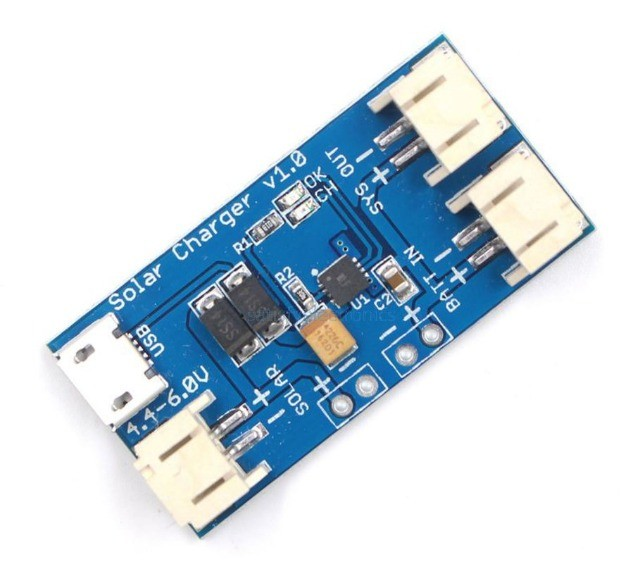
\includegraphics[width=0.3\textwidth]{figuras/cn3065} 
        \caption*{Fonte: AliExpress}
    \end{figure}

    O módulo (figura \ref{fig:cn3065}) possui entradas para carregamento, bateria, placa solar e saída para um circuito (nesse caso, o microcontrolador). 
    
    \subsection{Bateria Li-Íon 3,7V 5200mAh}
    A escolha da bateria foi feita considerando o tempo de uso da bateria, dado a corrente elétrica exigida pelos componentes, quanto pela compatibilidade com o módulo de carregamento. Assim, a bateria pode durar bastante tempo e, ainda, energizar todos os módulos do circuito.

     \begin{figure}[h!]
        \captionsetup{width=1\textwidth}
        \caption{\label{fig:bateria}Bateria Li-Íon 3,7V 5200mAh}
        \centering
        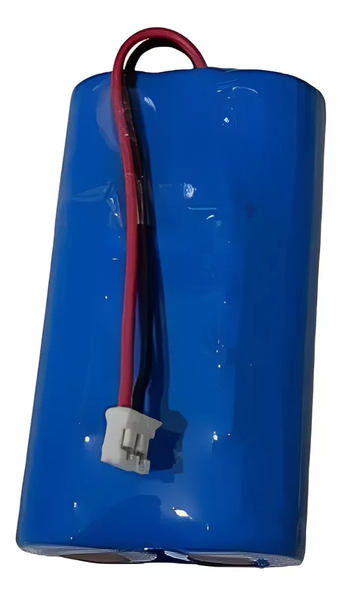
\includegraphics[width=0.2\textwidth]{figuras/bateria} 
        \caption*{Fonte: Mercado Livre}
    \end{figure}

    A Figura \ref{fig:bateria} ilustra o modelo escolhido, com um conector JST macho para o encaixe na entrada do módulo de carregamento CN3065.

    \section{Viabilidade Financeira}
    O sucesso de um projeto social não se mede apenas pelo impacto que ele gera na comunidade-alvo, mas também pela sua capacidade de se manter ao longo do tempo, sem depender exclusivamente do financiamento dos fundadores. Nesse contexto, a viabilidade financeira de nosso projeto assume um papel fundamental, pois buscamos criar um modelo sustentável que permita a continuidade das atividades sem gerar despesas ou desperdícios.

    Logo, é de suma importância analisar o valor mínimo para a criação da bengala, considerando inicialmente o custo dos materiais, para nortear as possíveis formas de expansão da bengala para o público-alvo.

    Primeiramente, é importante destacar que o frete não foi incluído nos custos de produção devido à existência prévia de algumas peças, as quais não tiveram seus preços para entrega registrados. Ainda assim, esses componentes foram incluídos na relação de valores para compra das peças. 

    Além disso, o tempo desempenhou um papel crucial na construção do projeto. Dada a importância de iniciar os testes e cumprir os prazos estabelecidos, priorizamos a compra dos materiais na mesma loja, buscando adquirir a maior quantidade possível de itens em um único local. Essa abordagem não apenas reduziu o tempo de entrega, mas também nos permitiu garantir que todos os componentes chegassem juntos, facilitando o início das atividades de teste.

    Para um projeto em escala real, a aquisição de itens em grande quantidade e a diversificação dos fornecedores podem ainda mais otimizar os custos. Com a compra em alta escala, é possível obter descontos significativos e negociar preços mais vantajosos. Além disso, ao ter diferentes distribuidores, podemos explorar opções de compra mais econômicas, fretes gratuitos a partir de valores mínimos na compra e reduzir ainda mais os custos totais dos componentes.
    
    O preço dos itens do protótipo ficou R\$148,40 para a produção do componente eletrônico da bengala. Nesse cálculo, foi desconsiderado o valor do frete, uma vez que alguns integrantes do grupo já possuíam certas peças que serviram para o desenvolvimento do trabalho, então não é possível incluir o valor para a entrega desses itens.

    Considerando todos esses aspectos, foi levantada uma relação dos valores reais de todos os componentes. O preço dos itens que não precisavam ser comprados foi estimado através da mesma loja utilizada para a compra dos sensores restantes para o projeto, como a protoboard, microcontrolador, fios e módulo de carregamento, que já haviam sido adquiridos anteriormente. Os valores de cada peça estão registrados no Quadro 6.


    \begin{quadro}[!ht]    
    \begin{center}
        
    \captionsetup{width=1.0\textwidth} % Definindo a largura da legenda
    \caption{Valor dos componentes essenciais}  
    \renewcommand{\arraystretch}{1.5} % Aumenta o espaçamento entre as linhas
    \begin{tabular}{lr}
        \toprule
        Componente & Valor (R\$) \\
        Microcontrolador UNO R3 com cabo USB & 37,50\\

        Bateria Li-Íon 3,7V 5200 & 29,90\\
        
        Módulo Carregamento CN3065& 18,90\\
        
        Módulo Buzzer Ativo 5V&4,90\\
        
        Chave DIP \texit{Switch} 1 Via&2,50\\
        
        Módulo Sensor \textit{Touch} Capacitivo TTP223B&2,90\\
        
        Módulo Sensor de Distância Ultrassônico HC-SR04 (2x)&25,80\\
        
        Módulo Motor de Vibração&10,90\\
        
        Fios encapados 0,75mm (2m de extensão)& 4,20\\
        
        Protoboard 400 Pontos& 10,90\\
        \bottomrule
    \end{tabular}
    \caption*{Fonte: elaborada pelos autores.} % Legenda sem rótulo

    \end{center}

\end{quadro}

     O valor total dos itens para a produção do componente eletrônico da bengala foi de R\$148,40, demonstrando um investimento inicial acessível para o desenvolvimento do projeto. Com a possibilidade de expansão para um projeto em escala real, a aquisição de itens em grande quantidade e a diversificação dos fornecedores oferecem oportunidades adicionais para otimizar os custos e garantir a sustentabilidade financeira a longo prazo.

     
    \subsection{Organizações para Parcerias}
    Introduzir parcerias estratégicas é fundamental para impulsionar a divulgação e distribuição das bengalas inteligentes para pessoas com deficiência visual. A iniciativa busca estabelecer colaborações com organizações não governamentais e entidades do setor público, com o objetivo duplo de ampliar o alcance do projeto e garantir recursos financeiros para sua continuidade e expansão. Essas parcerias não apenas possibilitam o oferecimento das bengalas para o público-alvo, mas também abrem oportunidades para arrecadação de fundos, viabilizando a compra de componentes e custeando o desenvolvimento contínuo da tecnologia. 

    
    \begin{itemize}
        \item \textbf{Centro de Apoio ao Deficiente Visual (CADEVI):} Organização sem fins lucrativos, fundada em 1984, com o propósito de auxiliar jovens e adultos que perderam a visão através da reintegração na sociedade. Nesse contexto, estreitar uma parceria com o CADEVI auxiliaria na distribuição da bengala entre pessoas que precisam de um auxílio especial para reaprender uma nova maneira de interagir com o espaço circundante.
        
        \item \textbf{Laramara:} Organização sem fins lucrativos, fundada em 1991, voltada a ações assistenciais com o intuito de promover vínculos sociais e desenvolver a autonomia dos indivíduos em diversas faixas etárias. Assim, através de atividades oferecidas a pessoas com deficiência visual, essa parceria torna-se benéfica pois a bengala pode passar a se tornar uma ferramenta utilizada no processo de desenvolvimento integral desse grupo.
        
        \item \textbf{Fundação Dorina Nowill:} Organização sem fins lucrativos com atuação na sociedade através de projetos sociais, produção de mídias físicas e digitais para pessoas com deficiência visual e consultoria de acessibilidade para empresas. Reconhecida por sua atuação na produção de mídias acessíveis e projetos sociais, a Fundação Dorina Nowill desempenha um papel fundamental na promoção da inclusão de pessoas com deficiência visual. Estabelecer uma parceria com a Fundação Dorina Nowill não apenas fortaleceria o projeto, mas também poderia abrir portas para colaborações em projetos de acessibilidade e consultoria, ampliando o impacto e a eficácia do nosso trabalho.
        
        \item \textbf{Secretaria Municipal da Pessoa com Deficiência (SMPED):} Criada em 2007 pela Lei Nº 14.659 em São Paulo, a SMPED tem sido uma importante parceira na promoção de políticas públicas de inclusão e acessibilidade. A Fundação Dorina Nowill já teve projetos financiados pela SMPED, o que evidencia a possibilidade de estabelecer uma colaboração para viabilizar financeiramente o desenvolvimento das bengalas inteligentes. Ao unir esforços com a SMPED, é possível aproveitar recursos públicos e auxílio financeiro para ampliar o alcance do projeto e beneficiar um maior número de pessoas com deficiência visual na comunidade.
    \end{itemize}

    \chapter{Execução do Projeto}

    Este capítulo apresenta um registro detalhado das atividades realizadas durante a execução do projeto, abrangendo desde o histórico das atividades até informações sobre a gestão e desenvolvimento. Serão discutidas as decisões tomadas ao longo do processo, incluindo escolhas técnicas, descartes de abordagens, os desafios enfrentados e superados e métricas de desenvolvimento. 

    \section{Histórico de Atividades}
    As atividades foram registradas no Jira e designadas aos integrantes responsáveis e, assim, marcadas como completas. Além disso, foram divididas em épicos, marcando cada uma das etapas principais do trabalho. As principais atividades estão detalhadas abaixo:

    \begin{itemize}
        \item Tarefas iniciais
        \begin{itemize} 
            \item Envio de formulários para criação do repositório no SVN
            \item Criação do blog 
            \item Criação do canal no YouTube
            \item Definição de cinco temas para o trabalho
        \end{itemize}
        \item Entrega 10/04
        \begin{itemize}
            \item Modelagem da bengala
            \begin{itemize}
                \item Tecnologias utilizadas
                \item Requisitos
                \item Necessidades atendidas
                \item O que a bengala irá fazer
                \item Estrutura física da bengala
            \end{itemize}
            \item Criação das histórias de usuário
            \item Documentação
            \item Definição de requisitos funcionais e não funcionais
            \item Vídeo da apresentação
            \item Criação dos slides
            \item Definição dos componentes utilizados
        \end{itemize}
        \item Entrega 17/04
        \begin{itemize}
            \item Compra dos componentes e sensores
            \item Prototipação da bengala 
                \begin{itemize}
                    \item Montagem do circuito no Tinkercad
                    \item Modelagem da bengala 
                \end{itemize}
        \end{itemize}
        \item Entrega 24/04
        \begin{itemize}
            \item Definição dos casos de teste de cada componente
            \item Desenvolvimento do código para testar os componentes
            \item Testes de funcionamento dos componentes
            \item Escrever sobre as conclusões
        \end{itemize}
        \item Entrega 10/05
        \begin{itemize}
            \item Integração de todos os componentes
            \item Incluir testes e prova de conceito na documentação
            \item Montagem do circuito
            \item Vídeo da apresentação
            \item Criação dos slides
        \end{itemize}
        \item Entrega 23/06
        \begin{itemize}
            \item Ajustes necessários na documentação
            \item Finalizar prototipação da bengala
            \item Definir viabilidade dos requisitos para o Produto Mínimo Viável
            \item Finalizar código para funcionamento dos componentes
        \end{itemize}
    \end{itemize}

    \section{Reuniões}

    Por conta da incompatibilidade de horários dos integrantes, as decisões foram feitas pessoalmente, em sala de aula, e no grupo de conversas online voltado para a discussão do projeto. Assim, decisões maiores foram realizadas pessoalmente, enquanto questões pontuais foram discutidas por mensagens.

    \section{Escolhas e Descartes}
    Inicialmente, foram diversas apuradas pelos integrantes acerca das funcionalidades da bengala. Por isso, algumas das ideias foram descartadas por incompatibilidade com os princípios do projeto. Como o baixo custo e o conforto do usuário na utilização da bengala foram priorizados, propostas que foram de encontro a esses pontos foram descartadas.

    O grupo considerou processamento de imagens para mapeamento de ambientes e leitura de placas como adição à identificação de objetos, contudo, essa funcionalidade exigiria a implementação de câmeras de qualidade e um microcontrolador com maior poder de processamento, memória e abertura a outras linguagens de programação. Assim, os custos do projeto aumentariam significativamente, dificultando a execução futura com um propósito social.

    Além disso, por ora, também foi descartada a conexão da bengala a dispositivos móveis. O descarte aconteceu pela decisão em manter a bengala independente, isto é, de forma que a utilização de suas funcionalidades não dependesse de nenhum aparelho externo ou conexão à Internet. 

    Portanto, manteve-se o foco em desenvolver uma bengala que pudesse detectar objetos, alertar o usuário de maneira efetiva e ter um bom desempenho em questão de durabilidade na bateria. Outro aspecto priorizado foi o conforto do usuário e design otimizado da bengala, de forma que a experiência do usuário durante o manuseio não fosse completamente diferente da utilização de uma bengala tradicional. Essa decisão foi tomada a fim de melhorar a adaptação durante o uso, considerando que a inclusão de componentes eletrônicos ao corpo do objeto o tornaria ligeiramente mais pesado que o comum.

    \section{Evolução do Projeto}
    Devido à greve, não houve maiores atualizações no projeto em termos de publicações e \textit{commits} no repositório. O Quadro abaixo ilustra o histórico total de commits, número de publicações no blog e vídeos ao longo dos meses. 

    \begin{quadro}[!ht]    
    \captionsetup{width=1.0\textwidth} % Definindo a largura da legenda
    \caption{Evolução do projeto ao longo dos meses}  
    \renewcommand{\arraystretch}{1.5} 
     \begin{tabular}{p{0.14\textwidth}p{0.14\textwidth}p{0.14\textwidth}p{0.14\textwidth}p{0.14\textwidth}p{0.14\textwidth}}
        \toprule
        Item & Março & Abril & Maio & Junho & Julho \\
        \midrule
        Commits & 2 & 15 & 22 & 22 & 29 \\
        Publicações & 4 & 8 & 10 & 10 & 11 \\
        Vídeos & 1 & 2 & 4 & 4 & 4 \\
        \bottomrule
    \end{tabular}
    \caption*{Fonte: elaborada pelos autores.} % Legenda sem rótulo
\end{quadro}

    O Apêndice \ref{ap:A} contém todas as publicações do blog, que descrevem com mais detalhes as tarefas realizadas semanalmente, dificuldades encontradas, decisões tomadas, dentre outras informações sobre o projeto. O Apêndice \ref{ap:B} contém também o endereço de acesso ao blog, ao canal e ao repositório.
	\chapter{Prova de Conceito}
\label{chap:prova-de-conceito}

A Prova de Conceito, ou Proof of Concept (POC), é um estágio crucial no desenvolvimento de qualquer projeto tecnológico. Ela consiste em uma fase dedicada a demonstrar a viabilidade e eficácia de uma ideia ou conceito inicial, fornecendo evidências tangíveis de que o projeto pode ser implementado com sucesso. Em essência, uma Prova de Conceito é uma espécie de teste preliminar, no qual protótipos ou modelos simplificados são criados e avaliados. Seu objetivo principal é validar a funcionalidade principal do conceito proposto, identificando potenciais desafios técnicos, explorando soluções alternativas e determinando a viabilidade do projeto em um contexto real.

\section{Implementação da Prova de Conceito}

Para realizar a Prova de Conceito da Bengala Inteligente, foi desenvolvido um protótipo inicial que integra todos os principais componentes do sistema. Isso incluiu a montagem física da bengala com os sensores e transdutores necessários, bem como a programação do microcontrolador para controlar o comportamento do dispositivo em resposta aos dados dos sensores.

\subsection{Montagem do Protótipo}

A montagem do protótipo envolveu a conexão dos sensores capacitivo de toque e ultrassônico no microcontrolador, de forma que eles pudessem captar dados de toque humano e da localização de objetos em relação ao sensor, garantindo uma demonstração prática para a detecção de obstáculos e interações táteis. 

Além disso, foi integrado um módulo de \textit{buzzer} para fornecer alertas sonoros ao usuário, bem como o motor de vibração para a indicação tátil ao usuário.

O circuito foi energizado diretamente pela bateria, ambos conectados entre si através do módulo de gerenciamento de energia. Com isso, tornou-se possível demonstrar a funcionalidade de recarregar através de uma fonte externa, bem como evitar sobrecargas durante a demonstração.

Por fim, a chave switch demonstrou a interrupção da corrente sendo conectada a um LED, de forma que possibilitou o controle mecânico acerca da luz estar acesa ou não. 


\subsection{Programação do Microcontrolador}

Utilizando um microcontrolador Arduino, foi desenvolvida a lógica de controle para processar os dados dos sensores e acionar os transdutores conforme necessário. Isso envolveu a configuração dos pinos de entrada e saída, a leitura dos dados dos sensores e a implementação de algoritmos para tomada de decisão com base nessas informações.

Os dados captados pelo sensor capacitivo são utilizados como critério para acionar o \textit{buzzer}, proporcionando uma resposta audível quando ocorre um toque. Essa escolha foi deliberada em consonância com o propósito central da bengala no que se refere à funcionalidade do sensor de toque. Embora o requisito primordial envolva a geração de alertas sonoros quando não houver toque por um período definido, indicando situações como queda da bengala, esquecimento de ligá-la ou perda, durante a demonstração seria impraticável manter o sensor constantemente ativado para evitar sons indesejados que poderiam interferir na apresentação. Portanto, optou-se por uma abordagem inversa, ou seja, ativar o \textit{buzzer} enquanto o toque estiver sendo detectado. Além disso, foi implementado um LED para que permanecesse ligado juntamente ao \textit{buzzer}.

Por outro lado, a escala de demonstração do sensor ultrassônico foi limitada para o raio de até 30 centímetros. Dessa forma, tornou-se possível demonstrar a variação do motor de vibração de forma mais evidente.

\section{Testes e Validação}

Após a montagem e programação do protótipo, foram realizados testes para validar a funcionalidade e eficácia do sistema. Isso incluiu testes de detecção de obstáculos usando os sensores de ultrassom, testes de sensibilidade do sensor capacitivo \textit{touch} e testes de resposta do \textit{buzzer}.

\subsection{Sensor ultrassônico}
O sensor ultrassônico emite ondas ultrassônicas de alta frequência através do pin Trigger, que são refletidas quando atingem um objeto e identificadas pelo sensor. Assim, o dado de recebimento da onda é enviado ao microcontrolador através do pino Echo. O cálculo de tempo e distância é feito a nível do software, considerando uma aproximação da velocidade do som no ar.

Notou-se, de maneira empírica, que o sensor tem uma dificuldade para identificar com precisão objetos pequenos. Entretanto, obteve-se um resultado satisfatório no quesito precisão em objetos maiores e velocidade da resposta.

\subsection{Buzzer Ativo}
O Buzzer foi utilizado para emitir sons sem diferenciação de frequência assim que o sensor capacitivo identificasse um toque. Utilizando um aplicativo de celular com o propósito de um decibelímetro, mensurou-se que a pressão sonora dos sons emitidos por este transdutor fica em torno de 60 dB, faixa aproximada de uma conversa normal. Apesar de ser alto, ainda permanece confortável ao ouvido humano.

\subsection{Motor de vibração}
O motor escolhido realiza até 9000 rotações por minuto (RPM), o que gera a sensação de vibração. A sua intensidade pode variar de 0 a 255, de acordo com o valor atribuído pelo toque. Embora a vibração mais forte seja bastante perceptível, ela fica bastante sutil conforme o número de rotações diminui. Todos os modos são perceptíveis pelo contato direto, contudo, a ideia é que o módulo seja integrado no corpo da bengala, então existe o risco de não haver uma distinção clara entre os alertas para objetos mais distantes. Por esse motivo, a prova de conceito revelou que é necessário explorar diferentes formas de reposicionamento do motor no corpo da bengala ou reavaliar opções que vibrem mais intensamente.

\subsection{Sensor capacitivo \textit{touch}}

O sensor capacitivo \textit{touch} é um dispositivo eletrônico que detecta a presença de um objeto condutor, como um dedo humano, sem a necessidade de contato físico direto. Ele opera com base na capacidade de detectar mudanças no campo elétrico ao redor do sensor quando um objeto se aproxima. Observou-se que ele possui uma resposta rápida ao toque, entretanto, ele detectou toques com uma distância de aproximadamente 3 milímetros (mm) do objeto condutor real (nesse caso, o dedo). Portanto, a detecção não acontece somente quando há um toque direto.

Além disso, ao ser tocado, o sensor capacitivo \textit{touch} mantém seu estado de saída alto por um período de aproximadamente 12 segundos (s). Dessa forma, mesmo que o objeto condutor permaneça em contato, o sensor deixará de identificar o toque após 12 segundos. Assim, volta a identificar com uma leve movimentação. 

Embora não seja completamente impreciso, apresenta características que se tornam aceitáveis, dado o contexto e os requisitos do projeto.






\subsection{Chave DIP Switch}
A chave DIP (Dual In-line Package) Switch é um componente eletrônico utilizado em circuitos integrados e placas de circuito impresso para configurar diferentes estados ou opções de funcionamento. Consiste em uma série de interruptores dispostos em uma linha, onde cada interruptor pode ser posicionado para estar aberto (desligado) ou fechado (ligado), permitindo configurar um conjunto de valores binários.

Apesar de ter cumprido com o objetivo proposto, a chave é bastante pequena e a sua movimentação é rígida, dificultando o manuseio. Com isso, tornou-se importante avaliar outras opções pensando na utilização por parte do usuário final.







\section{Resultados e Considerações}

Os resultados da Prova de Conceito demonstraram a viabilidade técnica da Bengala Inteligente, com uma integração eficaz dos componentes e uma resposta satisfatória aos estímulos externos. No entanto, foram identificados alguns pontos que requerem ajustes e melhorias, como a interação com componentes e a resposta de transdutores.

No geral, a Prova de Conceito foi bem-sucedida em validar a funcionalidade principal da Bengala Inteligente e fornecer percepções acerca dos componentes utilizados.


\chapter{PRODUTO MÍNIMO VIÁVEL}
O Minimum Viable Product (MVP), ou Produto Mínimo Viável, representa uma etapa crucial no ciclo de desenvolvimento de qualquer projeto tecnológico. É uma versão inicial e simplificada do produto final, projetada para validar as funcionalidades essenciais e coletar feedback inicial dos usuários. Ao contrário de uma versão completa, o MVP foca em oferecer apenas as funcionalidades básicas necessárias para resolver o problema principal do usuário. Este estágio permite não apenas testar a aceitação do produto, mas também validar o conceito, identificar ajustes necessários e refinar a estratégia de desenvolvimento.

\section{Implementação do Produto Mínimo Viável}
Para implementar o MVP da Bengala Inteligente, foi desenvolvido um protótipo inicial que se concentra nas funcionalidades fundamentais essenciais para melhorar a mobilidade e segurança dos usuários com deficiência visual. Dessa forma, decidiu-se que o projeto incluiria detecção de obstáculos, vibração ajustável, circuito desligável e com possibilidade de recarregar a bateria. Com isso, a bengala torna-se funcional ainda no estágio inicial de desenvolvimento.

\section{Prototipação da Bengala}
O modelo virtual da bengala foi prototipado considerando uma estrutura para alocação dos componentes, passagem de fios, leveza e ergonomia.

O protótipo foi realizado no Autodesk Inventor, software que permite criar protótipos virtuais tridimensionais e funcionais. Como partes integrantes da bengala, há a ponteira, um compartimento para alocação dos componentes eletrônicos e, por fim, a extensão.

A bengala mede 125,42cm e possui 1,6cm de diâmetro, permitindo um fácil manuseio da bengala por usuários de diferentes alturas. A espessura aumenta próximo à mão, medindo 2,0cm, o que permite maior conforto.

O Apêndice \ref{ap:C} ilustra diferentes ângulos do modelo tridimensional da bengala, detalhando as dimensões de cada componente.

\section{Componentes elétricos}
Os dois sensores ultrassônicos foram conectados ao microcontrolador, em conjunto com o módulo de motor de vibração. Além disso, o microcontrolador é alimentado pela bateria através do módulo de gerenciamento de carga (CN3065), com a chave DIP Switch interceptando a passagem de energia para permitir o desligamento do circuito. 

Foi desenvolvida uma função que monitora a atividade do sensor, convertendo o tempo em microssegundos para a distância entre o sensor e o objeto detectado. Assim, essa distância é utilizada para definir a intensidade de vibração do motor.

As condições definidas para o controle da vibração são baseadas na distância medida pelos sensores. Quando a distância detectada por qualquer um dos sensores é menor que 50 cm, o motor é acionado com uma intensidade máxima de vibração (255). Se a distância for menor que 100 cm, mas não tão próxima quanto 50 cm, a intensidade da vibração é reduzida para 200. Da mesma forma, distâncias inferiores a 150 cm acionam uma vibração moderada de intensidade 150. Se nenhuma das condições anteriores for atendida, o motor vibrará continuamente com uma intensidade mínima de 100.

Essas definições permitem ajustar a intensidade da vibração de acordo com a proximidade de obstáculos detectados, proporcionando feedback tátil adequado ao usuário para navegação segura e eficiente.

Além disso, é importante garantir que os atrasos (delays) inseridos após cada alteração na intensidade da vibração permitam que o feedback seja percebido de forma clara e oportuna pelo usuário, contribuindo para uma experiência de uso mais intuitiva e eficaz da bengala inteligente.


\section{Integração dos Componentes}
Na etapa do MVP, os componentes ainda não estão soldados num circuito integrado, uma vez que o projeto pode sofrer alterações que envolvem a inclusão, exclusão ou reestruturação das peças no circuito. Pensando nisso, os componentes estão integrados na parte externa da bengala com fita adesiva, ainda com a utilização da protoboard para auxiliar na montagem do circuito.

\section{Justificativa}
A escolha das funcionalidades presentes no MVP foi feita baseando-se no intuito primordial da bengala, bem como em aspectos não-funcionais que garantiriam uma boa experiência ao usuário durante a utilização desde o início.

 O Quadro abaixo revela os requisitos funcionais e não funcionais abrangidos na bengala. Assim, de 21 requisitos levantados inicialmente, 14 estão sendo implementados ainda na primeira versão (isto é, cerca de 66\%).
 
\begin{quadro}[!ht]    
    \captionsetup{width=1.0\textwidth} % Definindo a largura da legenda
    \caption{Requisitos gerais do MVP}  
    \renewcommand{\arraystretch}{1.5} % Aumenta o espaçamento entre as linhas
    \begin{tabular}{p{0.4\textwidth}p{0.54\textwidth}} % Definindo larguras para as colunas
        \toprule
        Referência & Nome  \\
        RF01 & Identificação de objetos   \\
        RF02 & Altura de objetos  \\
        RF03 & Detecção em ambientes escuros    \\
        RF04 & Modo de vibração   \\
        RF05 & Diferença entre os modos de vibração \\
        RF06 & Recarregamento da bengala   \\
        RF07 & Indicador de carga completa   \\
        RF08 & Desligamento  \\
        RNF01 & Tempo de vibração  \\
        RNF02 & Tempo de detecção \\
        RNF03 & Precisão   \\
        RNF05 & Entrada do carregador  \\
        RNF06 & Proteção contra sobrecarga   \\
        RNF07 & Autonomia de bateria  \\
        \bottomrule
    \end{tabular}
    \caption*{Fonte: elaborada pelos autores.} % Legenda sem rótulo
\end{quadro}

\section{Resultados e Considerações}

Após a implementação do MVP, foram obtidos resultados significativos que validam a funcionalidade e viabilidade do projeto inicial. O protótipo desenvolvido concentrou-se nas funcionalidades essenciais para melhorar a mobilidade e segurança dos usuários com deficiência visual. Isso incluiu a detecção de obstáculos, vibração ajustável, circuito desligável e recarregável, permitindo que a bengala se tornasse funcional desde o estágio inicial de desenvolvimento.

Os sensores ultrassônicos integrados ao microcontrolador demonstraram precisão satisfatória na detecção de objetos sólidos e na diferenciação de distâncias conforme especificado nos requisitos funcionais. O feedback tátil através da vibração foi implementado com sucesso, proporcionando uma comunicação clara das informações ambientais ao usuário durante a navegação.

Além disso, o módulo de gerenciamento de carga (CN3065) mostrou-se eficaz na recarga da bateria da bengala, garantindo uma autonomia adequada para o uso diário. Esse aspecto é crucial para assegurar que o dispositivo seja prático e confiável para os usuários em suas atividades cotidianas.

Em termos de validação do conceito, o MVP foi bem-sucedido em demonstrar que as funcionalidades propostas podem resolver efetivamente os desafios enfrentados pelos usuários com deficiência visual. 
	%\chapter{Conclusões e Trabalhos Futuros}
\label{chap:conclusoes-e-trabalhos-futuros}

Parte final do texto na qual se apresentam as conclusões apoiadas no desenvolvimento do assunto. É a recapitulação sintética dos resultados obtidos. Pode apresentar recomendações e sugestões para pesquisas futuras.

%\label{sec:contribuicoes-do-trabalho}



%\label{sec:limitacoes}








	
	%Elementos pós-textuais	
	\bibliography{3-pos-textuais/referencias}
%	\imprimirglossario %	
	%\imprimirapendices
		% Adicione aqui os apendices do seu trabalho
	%	\apendice{POSTAGENS NO BLOG}
\label{ap:A}

\section{Semana 1 (06/03/2024) - Apresentação da disciplina }
Na semana passada, no dia 28/02, tivemos nossa primeira aula de PI1A5 com o Professor Johnata. Embora ainda não tenhamos feito decisões específicas sobre o projeto, o professor nos apresentou a disciplina e explicou o que será esperado de nós nas próximas aulas, além de detalhar as próximas entregas e como deverão ser feitas. 

Com base nessas informações, começamos a considerar possíveis temas para o projeto e iniciamos pesquisas preliminares.

\section{Semana 2 (13/03/2024) - Formação dos grupos }

 Após a apresentação inicial da disciplina, nós formamos o nosso grupo com seis integrantes e decidimos o nosso nome Patent Pending.

A ideia surgiu, ironicamente, por estarmos sem ideia de qual nome representaria perfeitamente a equipe e o tema que ainda não havia sido definido. Logo, optamos por uma patente pendente.

Com a definição de quem seriam os integrantes, foi definido que a nossa ferramenta principal de organização seria o Jira. Dessa forma, a separação de tarefas e visualização de prazos fica mais facilitada por ser uma ferramenta voltada ao gerenciamento de projetos.

Alguns tópicos apresentados na primeira aula já foram convertidos em tarefas pendentes, tais como criação deste blog, novo canal no youtube e pesquisa de temas possíveis.

\section{Semana 2 (20/03/2024) -  Discussão sobre os temas }
Nessa última semana, nós começamos a discutir os possíveis projetos que gostaríamos de desenvolver ao longo da disciplina nesses dois últimos semestres.

Entre dez temas iniciais, sugeridos pelos integrantes do grupo, nós escolhemos as cinco melhores ideias para discutir com o professor a respeito da viabilidade.

As nossas sugestões incluíram uma plataforma para contratação de artistas, comunidade virtual para leitores, ferramenta para gerenciamento do processo de estágio entre aluno e universidade, aplicação para controle financeiro e, por fim, uma bengala inteligente.

Após a discussão com o professor, optamos por desenvolver a bengala inteligente. As escolhas individuais não formaram um consenso, portanto, foi necessário argumentar os prós e contras de cada tema e partir da decisão da maioria.

A escolha final foi feita, sobretudo, pela relevância do tema e inovação do projeto. A bengala é voltada para pessoas com deficiência visual e, atualmente, não existem ferramentas acessíveis no mercado voltada a essa população. Após realizarmos uma pesquisa de mercado, notamos que não existem outras tecnologias assistivas focadas em manter um custo baixo e ir além de uma bengala comum.


\section{Semana 4 (27/03/2024)  - Apresentação do tema }

Iniciamos as pesquisas iniciais sobre o tema, argumentando sobre a viabilidade do projeto, relevância do tema, pesquisas sobre o assunto e propostas de funcionalidades.

Ao montar a apresentação para introduzir o nosso projeto à sala, utilizamos o LaTeX pela primeira vez com o intuito de estruturar os slides. Apesar da dificuldade inicial, utilizar o modelo pronto fornecido pelo professor facilitou bastante esse primeiro contato. Além disso, o fato do Overleaf proporcionar ferramentas que permitem facilmente assimilar o conteúdo textual com a parte correspondente no PDF auxiliou a compreender o que cada tag fazia.

Uma dificuldade deu-se pelo fato de que a compilação no Overleaf era constantemente interrompida por conta do limite de tempo estabelecido na versão gratuita. Após algumas tentativas de recompilação, dava certo. Ainda assim, foi um pequeno empecilho durante o desenvolvimento dos slides.

Nós apresentamos o projeto para a turma e, em seguida, recebemos feedback do professor acerca da apresentação. Um ponto positivo foi a evidente pesquisa que fizemos para poder argumentar e explicar sobre o tema, contudo, foi recomendado que não nos estendêssemos tanto para não tangenciar demais o assunto e acabar passando do tempo limite.

Para a próxima entrega, devemos também voltar a pesquisa para trazer outros trabalhos acadêmicos que tenham desenvolvido o mesmo projeto. A ideia é que possamos usar como referência e também apontar diferenciais da nossa sugestão.



\section{Semana 5 (03/04/2024)  - Refinamento da ideia }
Algumas decisões importantes foram feitas acerca da bengala, quais seriam as principais funcionalidades e os requisitos. 

Dessa forma, a equipe trabalhou em desenvolver as histórias de usuário do projeto e seus respectivos critérios de aceitação. Com esses pontos prontos, ficou mais fácil definir quais seriam os requisitos funcionais e não funcionais que atendessem a essas funcionalidades desejáveis. 

O desenho técnico do projeto foi iniciado, bem como o estudo do possível design da bengala considerando a maneira que pessoas com deficiência visual já utilizam bengalas convencionais. O propósito é que a bengala inteligente seja um substituto viável a alternativas analógicas comuns, portanto, foi importante pensar numa forma de preservar a mesma leveza e ergonomia.

A documentação do projeto também foi iniciada, trazendo a introdução do projeto e estudo das alternativas existentes no mercado. 

Houve discussões acerca da viabilidade das nossas propostas iniciais, sendo elas a integração com um aplicativo o principal desafio por questão de tempo e falta de familiaridade por parte do grupo com essa área de desenvolvimento. A possibilidade de não ter um aplicativo agora apresentou empecilhos para outras funcionalidades anteriormente idealizadas, como localização da bengala, reconhecimento de imagem e integração com um mapa para cálculo de rotas. 

Outra alternativa para manter algumas funcionalidades rodando localmente seria o uso de um microcontrolador mais potente, como Raspberry PI em vez de Arduino, uma vez que este último possui limitações de processamento, memória e linguagem de programação. Contudo, a escolha de um outro microcontrolador resulta no aumento de custos do projeto, nos levando a escolher o foco em outras funcionalidades por enquanto.


\section{Semana 6 (10/04/2024) - Desenho da aplicação }
 Na última semana, tivemos a oportunidade de discutir com o professor sobre as possíveis funcionalidades da bengala. Como o nosso objetivo é manter os custos baixos para tornar a ferramenta acessível, utilizar microcontroladores com maior poder de processamento e mais memória não é viável por enquanto.

No sábado, o grupo se reuniu para definir qual seria a segunda funcionalidade principal, além de definir melhor os responsáveis por cada segmento do projeto. Apesar de concordarmos com uma flexibilidade na designação de tarefas, foi importante decidir responsáveis por cada parte do trabalho para que fosse possível evitar a centralização de diversas atividades em poucas pessoas. Além disso, também permite uma gestão melhor, já que existem pessoas específicas pensando em todas as frentes de desenvolvimento.

Na reunião, alinhamos que a funcionalidade secundária escolhida seria a detecção do toque do usuário na bengala, de forma que ela emitisse alarme sonoro/vibratório após um longo período de inatividade na região do apoio de mão. Isso permite que o usuário possa desligar a bengala, se necessário, ou localizá-la facilmente no ambiente caso tenha perdido ou esquecido de pegá-la.

Foram feitos testes de componentes no Tinkercad, com a demonstração da vibração da bengala de acordo com a distância do objeto identificado. O uso de dois sensores ultrassônicos foi testado numa simulação a parte. Além disso, a modelagem 3D também foi realizada no mesmo software, escolhido pela possibilidade de montar circuitos virtualmente e uma ampla disponibilidade de componentes e peças. 

Contudo, apesar da amplitude de escolhas, o Tinkercad não oferece todos os componentes que escolhemos utilizar no nosso projeto. Assim, os componentes foram comprados na semana passada e possuem previsão de chegar nessa semana. Com isso, será possível testar a comunicação de mais sensores ao mesmo tempo, até que todos sejam integrados num único circuito no projeto finalizado.

A documentação foi finalizada também na última semana, bem como a apresentação em slides. Durante a apresentação do desenho da aplicação, levamos em consideração os pontos de melhora sugeridos pelo professor, como tempo de fala, quantidade de texto em slides e excesso de detalhes acerca de temas fora do escopo. Com isso, notou-se uma melhora significativa na qualidade geral da apresentação.

Assim que os componentes chegarem, será possível testá-los para que possíveis problemas nas peças sejam identificados e corrigidos a tempo da próxima apresentação.

\section{Semana 7 (17/04/2024) - Definição de teste dos componentes }
Na última aula, o professor especificou o que seria esperado da prova de conceito e dos testes de componentes. Assim, definimos quais aspectos dos componentes nós testaríamos e quais seriam os parâmetros desses testes.

Vamos utilizar algumas planilhas disponibilizadas para especificar cada um dos testes. Os que nós decidimos, até então, são:

1.  Sensor ultrassônico

    a. Distância mínima e máxima de detecção

    b. Variação da distância detectada pelo código e pela mensuração

    c. Ângulo de detecção

2. Motor de vibração

    a. Vibração mínima e máxima

3. Buzzer

    a. Decibéis do som emitido

4.  Sensor de toque

    a. Tempo máximo de toque contínuo para continuar detectando

    b. Tempo mínimo de toque para o reconhecimento

    c. Área de detecção do toque no sensor

    d. Outros objetos que ativam o toque

5. Bateria

    a. Possibilidade de energizar o microcontrolador com todos os componentes ao mesmo tempo

    b. Duração da bateria durante o uso contínuo

6.  Módulo de carregamento

    a. Carregamento da bateria sem esquentar

    b. Tempo de carregamento de acordo com a capacidade da bateria


Um obstáculo, até então, reside na dificuldade para medir com exatidão alguns componentes, a fim de deixar o teste mais preciso. O motor de vibração, por exemplo, precisa de um parâmetro para indicar que a sua resposta tátil é forte o suficiente quando estiver acoplada no corpo de uma bengala. Além disso, medir o nível de carregamento da bateria é difícil e pode não ser tão específico sem uma ferramenta específica.

\section{Semana 8 (24/04/2024) - Integração dos componentes }
Os componentes chegaram e foi possível testá-los individualmente e em conjunto. Descobrimos que o buzzer ativo possui um som muito alto e, por não permitir a alteração de frequência, pode ser um pouco incômodo durante a utilização. 

A bateria está funcionando normalmente e foi possível energizar todos os componentes ao mesmo tempo. Além disso, o módulo de carregamento indica o carregamento da bateria através de uma luz de LED acesa. 

O motor de vibração vibra bem, variando de 0 a 255 em intensidade, mas os níveis mais baixos podem ser imperceptíveis ao usuário quando o sensor for acoplado na bengala. Assim, precisamos realizar mais testes para determinar onde o motor deve ficar para que a vibração seja amplificada ou decidir se outros motores em conjunto serão necessários.

Os sensores ultrassônicos identificam objetos até uma boa distância, então o propósito será atendido. Apenas precisamos nos certificar de que ele é suficientemente preciso e consegue identificar objetos de diferentes alturas e tamanhos.

\section{Semana 9 (01/05/2024) - POC }
Iremos apresentar a prova de conceito na próxima semana. Assim, terminamos a apresentação de slides e definimos o escopo do que será apresentado à turma. 

Realizaremos a apresentação do funcionamento real dos transdutores (motor de vibração e buzzer) e sensores (capacitivo e ultrassônico). Assim, vamos criar um código específico para essa etapa a fim de acoplar todos os componentes:

1. Quando o sensor capacitivo identificar um toque, o buzzer ativará por alguns instantes.

    a. Demonstração da captação do toque e da resposta sonora

2. Dependendo da distância do objeto identificado pelo sensor ultrassônico, o motor vibrará mais ou menos.

    a. Demonstração da variação de vibração e da amplitude da distância detectada
    
\section{Semana 10 (08/05/2024) - Apresentação da POC }
 A prova de conceito foi apresentada para a turma hoje. A apresentação incluiu a introdução de todos os componentes integrados num circuito, de forma que a funcionalidade de todos pudesse ser testada e representada.

Assim, o código foi desenvolvido a fim de obter respostas de todos os sensores e, concomitantemente, estimular os transdutores.



\section{Semana 11 (17/07/2024) - Pós greve e finalização do documento}
Durante a terceira semana de maio, o professor da disciplina entrou em greve, a qual encerrou-se no dia 28 de junho. Assim, nossas aulas retornaram como período de reposição após o período de férias (01/07 até 15/07). 

Tivemos a nossa primeira aula após esse período hoje, na qual discutimos os futuros prazos de entrega e apresentações para finalização do quinto semestre. Dessa forma, o documento deverá ser entregue até o dia 23/07 com todos as informações até o MVP.

Em seguida, no dia 24/07, haverá a preparação para a apresentação que está prevista de ocorrer no dia 31/07. Com o trabalho apresentado para a banca, as alterações serão enviadas até o dia 07/08.

Recebemos feedback do professor quanto à documentação existente, com as seguintes sugestões de alteração antes da entrega:

- Incluir textos antes e depois de cada tabela, quadro, imagem ou lista dentro do documento

- Referenciar os itens acima no texto, garantindo que eles estejam associados com o que está escrito

- Alterar as tabelas para quadros

- Incluir referências no texto dos dados trazidos durante a argumentação



Junto com os pontos mencionados acima, será adicionada ao documento a seção de apresentação do MVP.

	%	\apendice{Acesso aos canais do projeto}
\label{ap:B}

    \begin{figure}[h!]
        \captionsetup{width=1\textwidth} 
        \caption{\label{fig:qr_bog} QR Code do blog Patent Pending }
        \centering
        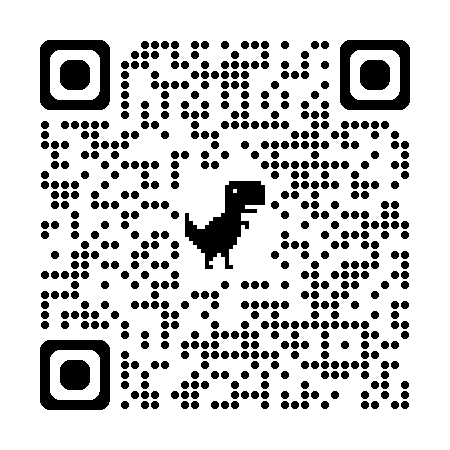
\includegraphics[width=0.7\textwidth]{figuras/qr_bog.png} 
        \caption*{Fonte: eladorada pelo autor.}
    \end{figure}

        \begin{figure}[h!]
        \captionsetup{width=1\textwidth} 
        \caption{\label{fig:qr_canal} QR Code do canal Patent Pending }
        \centering
        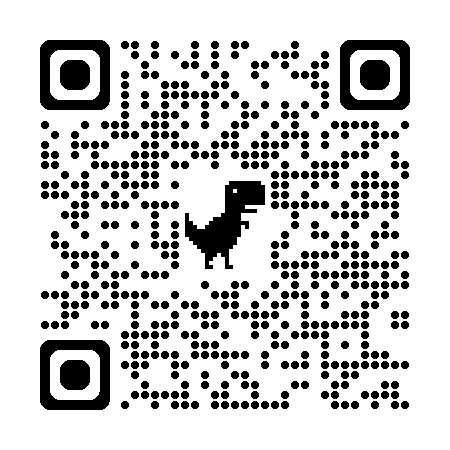
\includegraphics[width=0.7\textwidth]{figuras/qr_canal.png} 
        \caption*{Fonte: eladorada pelo autor.}
    \end{figure}

        \begin{figure}[h!]
        \captionsetup{width=1\textwidth} 
        \caption{\label{fig:qr_git} QR Code do repositório Patent Pending }
        \centering
        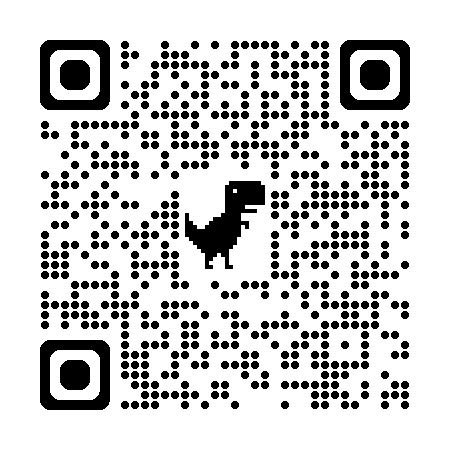
\includegraphics[width=0.7\textwidth]{figuras/qr_git.png} 
        \caption*{Fonte: eladorada pelo autor.}
    \end{figure}
	%	\apendice{PROTOTIPAÇÃO DA BENGALA}
\label{ap:C}

As imagens referem-se à modelagem e dimensões dos componentes do corpo da bengala, desenvolvidos para construção com filamentos em impressora 3D.

    \begin{figure}[h!]
        \captionsetup{width=1\textwidth}
        \caption{\label{fig:prototipo1} Visão lateral do protótipo }
        \centering
        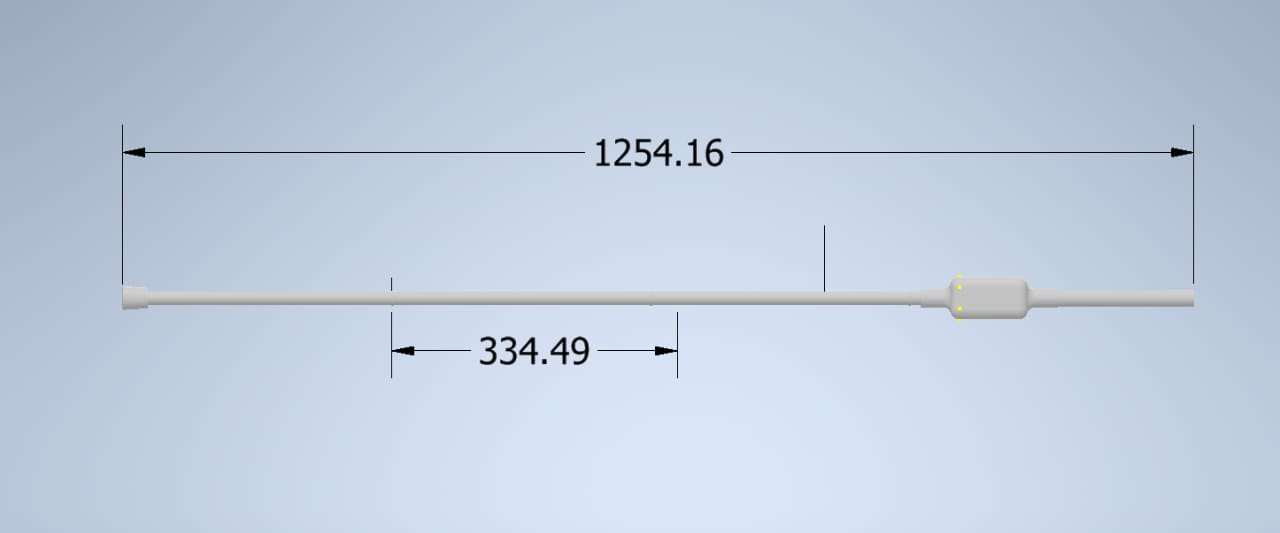
\includegraphics[width=0.7\textwidth]{figuras/prototipo1.jpeg} 
        \caption*{Fonte: eladorada pelo autor.}
    \end{figure}

    \begin{figure}[h!]
        \captionsetup{width=1\textwidth}
        \caption{\label{fig:prototipo2} Visão superior do protótipo}
        \centering
        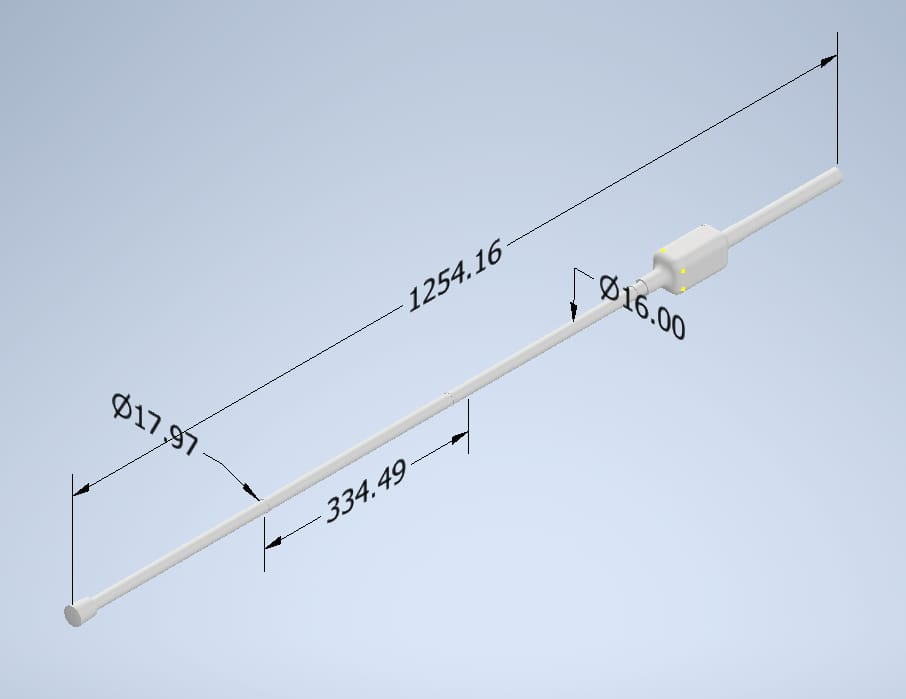
\includegraphics[width=0.7\textwidth]{figuras/prototipo2.jpeg} 
        \caption*{Fonte: eladorada pelo autor.}
    \end{figure}

        \begin{figure}[h!]
        \captionsetup{width=1\textwidth}
        \caption{\label{fig:prototipo3}Detalhamento do espaço para os componentes}
        \centering
        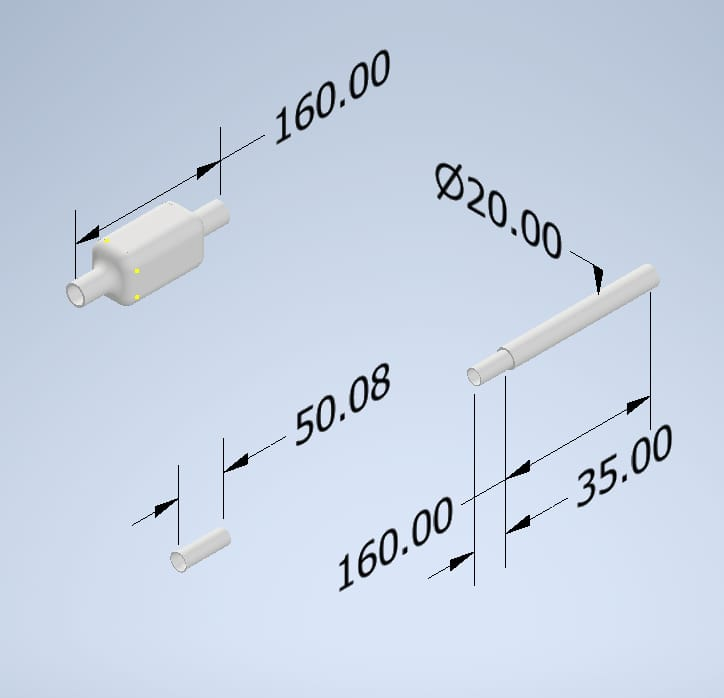
\includegraphics[width=0.7\textwidth]{figuras/prototipo3.jpeg} 
        \caption*{Fonte: eladorada pelo autor.}
    \end{figure}
		
	%	\imprimiranexos
		% Adicione aqui os anexos do seu trabalho
	%	\anexo{ Exemplo de um anexo em PDF}
\label{an:ex_anexo_b}

O autor pode anexar um \gls{PDF}, traduzido como formato portátil de documento. Veja o código fonte utilizado para anexar o arquivo ``Sikasil.pdf'' que foi colocado dentro da pasta ``anexos'' que por sua vez está dentro da pasta ``elementos-pos-textuais''. Tenha muita atenção na hora de especificar o local do arquivo. Recomenda-se não utilizar caracteres especiais para nomear pastas e, principalmente, arquivos. 

Pode-se fazer uma descrição sucinta do arquivo anexado.

%Comando para incluir um arquivo em PDF:
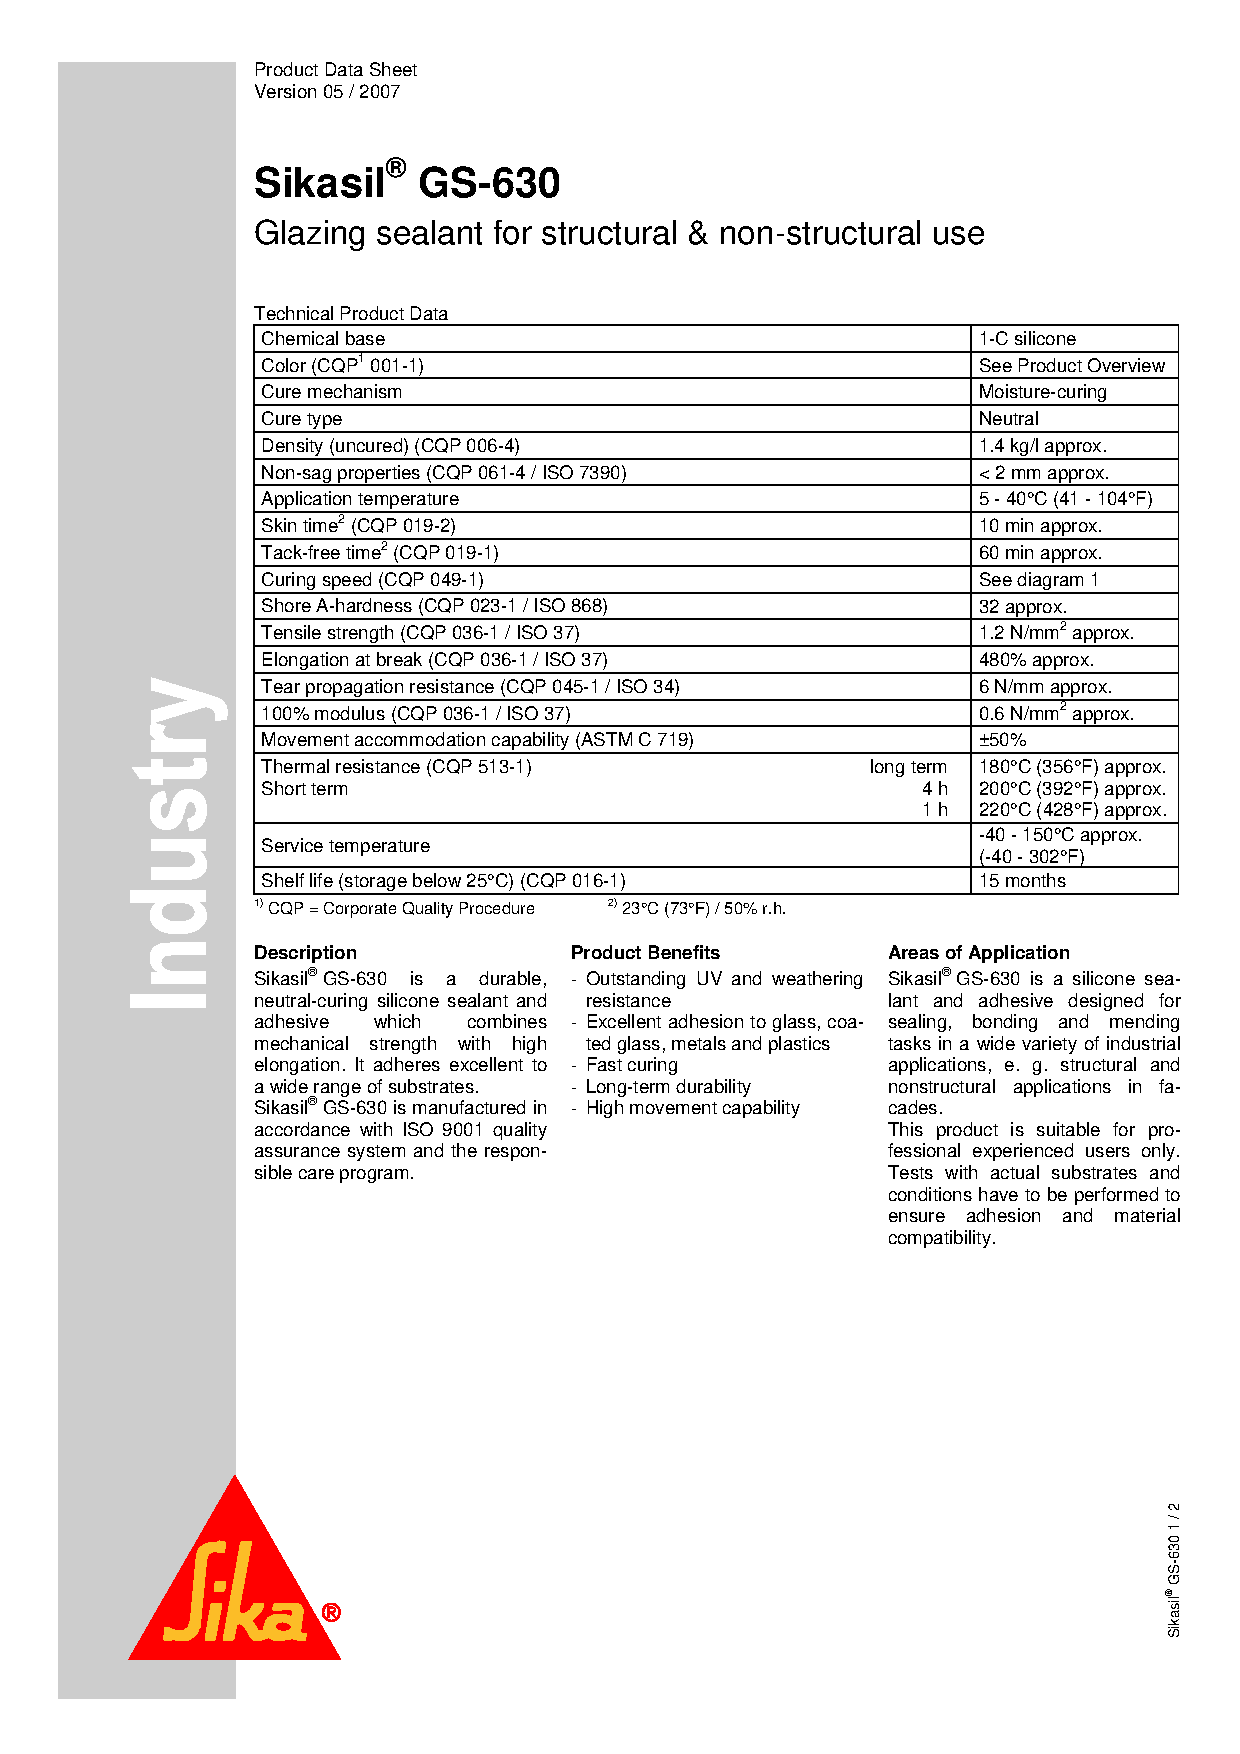
\includepdf[pages={-}]{3-pos-textuais/anexos/Sikasil.pdf}

		
    %\imprimirindice
    
	

\end{document}
